% =====================================================================
%  Sistema Nacional/Regional de Gestion de Respuesta a Desastres
%  Naturales y Asignacion Resiliente de Recursos
%  Compilar con:  pdflatex sistema_gestion_desastres.tex  (x2)
% =====================================================================
\documentclass[11pt,a4paper]{article}

\usepackage[utf8]{inputenc}
\usepackage[T1]{fontenc}

% Español. Si tu instalación no trae babel-spanish, se usan los rótulos manuales.
\IfFileExists{spanish.ldf}{%
  \usepackage[spanish,es-noquoting,es-tabla]{babel}%
}{%
  \renewcommand{\contentsname}{Índice}%
  \renewcommand{\tablename}{Tabla}%
  \renewcommand{\figurename}{Figura}%
  \renewcommand{\abstractname}{Resumen}%
  \renewcommand{\listfigurename}{Índice de figuras}%
}
% microtype requiere fuentes escalables (lmodern), por eso van juntos.
\IfFileExists{lmodern.sty}{%
  \usepackage{lmodern}%
  \IfFileExists{microtype.sty}{\usepackage{microtype}}{}%
}{}

\usepackage[margin=2.5cm]{geometry}
\usepackage{graphicx}
\usepackage{float}
\usepackage{pdflscape}
\usepackage{booktabs}
\usepackage{tabularx}
\usepackage{enumitem}
\usepackage{parskip}
\usepackage[hidelinks]{hyperref}

\hypersetup{
  pdftitle={Sistema Nacional/Regional de Gestion de Respuesta a Desastres Naturales y Asignacion Resiliente de Recursos},
  pdfsubject={Arquitectura empresarial y tecnologica para la coordinacion interinstitucional}
}

% Columna X centrada verticalmente para las tablas
\newcolumntype{L}{>{\raggedright\arraybackslash}X}

\title{\textbf{Sistema Nacional/Regional de Gestión de Respuesta a Desastres
Naturales y Asignación Resiliente de Recursos}\\[0.4em]
\large\normalfont\itshape Propuesta de arquitectura empresarial y tecnológica
para la coordinación interinstitucional}

\author{Juan Esteban Cruz \and Deisy Lorena Guzmán \and Sebastián Villarraga \\[0.3em]
\small Arquitecturas Empresariales (AREP) --- Escuela Colombiana de Ingeniería Julio Garavito}
\date{\today}

\begin{document}

\maketitle

\begin{abstract}
\noindent
Los desastres naturales exigen decisiones coordinadas entre múltiples
organizaciones que operan con sistemas, datos y procedimientos propios.
Este documento propone una arquitectura empresarial interoperable,
resiliente y apoyada en inteligencia artificial y optimización matemática,
concebida como un \emph{System of Systems}, para transformar información
heterogénea y distribuida en decisiones operativas oportunas, optimizadas y
trazables durante la respuesta a emergencias. La arquitectura se documenta con
el modelo C4 --- contexto, contenedores, componentes y despliegue --- junto con
las decisiones arquitectónicas que la sustentan y su trazabilidad con las capas
de arquitectura empresarial. A partir de ella se delimita y construye un
prototipo del nodo \emph{edge} municipal, implementado en Java con Spring Boot:
ingesta IoT por MQTT, detección de eventos y alertas en tiempo real,
almacenamiento local con patrón \emph{outbox}, sincronización idempotente con
la nube y auditoría encadenada.
En un escenario simulado de 6\,000 lecturas con una caída de 40\,s del enlace,
el nodo \emph{edge} mantuvo una latencia de alerta p95 de 42\,ms, detectó los
24 episodios planteados y no perdió ni duplicó lecturas, mientras que una línea
base solo nube perdió el 33,5\,\% de las lecturas y 10 de los 12 episodios
ocurridos durante la caída. Los resultados se mantuvieron al desplegar la nube
en AWS, con el enlace sobre internet real.
\end{abstract}

\tableofcontents
\listoffigures
\bigskip

% =====================================================================
\section{Contexto y problema}
% =====================================================================

Los desastres naturales generan impactos simultáneos sobre población,
infraestructura, servicios públicos, vías y actividades económicas.
Inundaciones, movimientos en masa, incendios forestales, terremotos y
crecientes súbitas pueden afectar varios municipios al mismo tiempo,
haciendo insuficiente la capacidad de respuesta de una sola organización.

En Colombia, la gestión del riesgo se desarrolla mediante el Sistema Nacional
de Gestión del Riesgo de Desastres (SNGRD), que articula entidades públicas,
privadas y comunitarias. La UNGRD cumple funciones de coordinación. A nivel
internacional, el Marco de Sendai 2015--2030 plantea como prioridades
comprender el riesgo, fortalecer la gobernanza, invertir en resiliencia y
mejorar la preparación y recuperación.

Según los datos utilizados en esta propuesta, durante 2025 se registraron más
de 4.700 emergencias en 869 municipios y más de 285.100 familias afectadas.
Estas cifras muestran que la respuesta requiere coordinación a una escala que
supera a una organización individual.

El problema central no es la ausencia de instituciones o tecnologías, sino la
dificultad para transformar información heterogénea y distribuida en
decisiones operativas coordinadas, oportunas, optimizadas y trazables. Durante
una emergencia participan organismos de socorro, gobiernos, salud, seguridad,
servicios públicos, organizaciones humanitarias y proveedores logísticos, cada
uno con sistemas y procedimientos propios.

Esta fragmentación puede producir información duplicada, diferentes niveles de
actualización, retrasos en la identificación de necesidades, asignaciones
ineficientes, dificultades para adaptar rutas y problemas para reconstruir
posteriormente las decisiones. La cadena crítica puede resumirse como:

\begin{center}
evento $\rightarrow$ detección $\rightarrow$ evaluación $\rightarrow$
necesidades $\rightarrow$ priorización $\rightarrow$ asignación $\rightarrow$
logística $\rightarrow$ ejecución $\rightarrow$ seguimiento $\rightarrow$
auditoría.
\end{center}

Por ello, la propuesta no se plantea como una aplicación móvil aislada, sino
como una capacidad transversal de mando, coordinación e integración
interinstitucional.

% =====================================================================
\section{Motivación y pregunta de investigación}
% =====================================================================

\subsection{Motivación}

Cuando ocurre un desastre, conocer dónde ocurrió el evento es solo el primer
paso. Las autoridades necesitan determinar qué zonas requieren atención
prioritaria, qué recursos están disponibles, qué rutas permanecen operativas,
cuánto suministrar y cómo coordinar a los diferentes actores. Estas decisiones
deben tomarse con información incompleta y cambiante.

Desde la Arquitectura Empresarial, esto representa un problema de alineación
entre negocio, información, aplicaciones y tecnología. La solución debe
permitir que las organizaciones mantengan sus capacidades existentes y, al
mismo tiempo, compartan información y coordinen decisiones mediante servicios
comunes.

\subsection{Pregunta de investigación}

\begin{quote}
\itshape
¿Cómo puede una arquitectura empresarial interoperable, resiliente y apoyada
en inteligencia artificial y optimización matemática mejorar la coordinación
interinstitucional y la asignación de recursos durante la respuesta a
desastres naturales?
\end{quote}

\subsection{Indicadores}

\begin{itemize}[leftmargin=*]
  \item Tiempo desde la detección hasta la evaluación.
  \item Tiempo desde la evaluación hasta la asignación.
  \item Porcentaje de solicitudes atendidas dentro del tiempo objetivo.
  \item Kilómetros y costos asociados a las operaciones logísticas.
  \item Porcentaje de demanda satisfecha y población prioritaria atendida.
  \item Porcentaje de operaciones que pueden mantenerse con conectividad
        degradada.
  \item Porcentaje de decisiones y recursos con trazabilidad completa.
\end{itemize}

% =====================================================================
\section{Estado del arte}
% =====================================================================

La propuesta combina varias líneas de investigación que ya han abordado partes
del problema. El vacío no está en la inexistencia de soluciones, sino en
integrarlas dentro de una arquitectura orientada a la operación.

\begin{table}[htbp]
\centering
\caption{Líneas de investigación relacionadas, aportes y limitaciones.}
\label{tab:estado-arte}
\begin{tabularx}{\textwidth}{@{}p{3.4cm}LL@{}}
\toprule
\textbf{Línea} & \textbf{Aporte} & \textbf{Limitación} \\
\midrule
Interoperabilidad & Integra organizaciones y sistemas heterogéneos. &
Requiere estándares y gobernanza. \\
\addlinespace
GIS y observación de la Tierra & Representa el impacto territorial. &
No determina por sí sola la mejor asignación. \\
\addlinespace
IA para daños & Acelera la evaluación preliminar. &
Depende de datos y validación. \\
\addlinespace
Logística humanitaria & Optimiza inventarios, localización y distribución. &
Muchos modelos usan escenarios específicos. \\
\addlinespace
Optimización de rutas & Reduce tiempos y costos. &
Necesita información actualizada. \\
\addlinespace
Sistemas resilientes & Mantienen funciones con conectividad limitada. &
La sincronización es compleja. \\
\addlinespace
Gobernanza & Aporta control y transparencia. &
Debe integrarse a la operación. \\
\bottomrule
\end{tabularx}
\end{table}

\subsection{Interoperabilidad}

Los estudios sobre gestión de desastres identifican la interoperabilidad, la
cooperación y la integración tecnológica como retos persistentes. Esto
respalda una capa común que conecte sistemas existentes sin exigir su
sustitución inmediata.

\subsection{Información geoespacial}

La observación de la Tierra y los sistemas GIS permiten relacionar el evento
con población, infraestructura, vías y recursos. Servicios como Copernicus
Emergency Management Service muestran que esta información ya se utiliza en
emergencias. El reto adicional es convertirla en decisiones logísticas.

\subsection{Inteligencia artificial}

Los modelos de aprendizaje profundo pueden localizar edificaciones y estimar
niveles de daño mediante imágenes. Sin embargo, su rendimiento puede variar
según el desastre, las imágenes disponibles y el territorio. Por ello, la IA
debe generar evaluaciones preliminares que puedan ser revisadas por los
responsables.

\subsection{Optimización y logística humanitaria}

La investigación en logística humanitaria aborda localización de centros,
inventarios, asignación, evacuación y ruteo bajo incertidumbre. La oportunidad
de esta propuesta está en conectar estos modelos con datos operativos que
cambian continuamente.

\subsection{Gobernanza}

La respuesta también depende de quién puede decidir, consultar información y
disponer de recursos. La arquitectura debe incorporar control de acceso,
trazabilidad, auditoría, responsabilidad y protección de información desde el
diseño.

% =====================================================================
\section{Propuesta de solución}
% =====================================================================

Se propone un Sistema Nacional/Regional de Gestión de Respuesta a Desastres y
Asignación Resiliente de Recursos, concebido como un \emph{System of Systems}.
Su objetivo es integrar datos, organizaciones, procesos y capacidades
tecnológicas para apoyar decisiones coordinadas.

\subsection{Fuentes de información}

La plataforma recibiría información de sensores, estaciones meteorológicas,
imágenes satelitales, drones, GIS, censos, infraestructura crítica, reportes
de organismos de socorro, inventarios, vehículos, hospitales, vías y
pronósticos meteorológicos.

\subsection{Integración e interoperabilidad}

Esta capa actuaría como punto común entre sistemas institucionales. Su flujo
básico sería: recibir $\rightarrow$ normalizar $\rightarrow$ validar
$\rightarrow$ georreferenciar $\rightarrow$ distribuir. Se podrían emplear
APIs, eventos, middleware y estándares de intercambio. El principio
arquitectónico es integrar antes que reemplazar.

\subsection{Inteligencia y analítica}

La IA apoyaría la detección de daños, clasificación de zonas afectadas,
estimación preliminar del impacto, identificación de infraestructura crítica y
generación de alertas. Paralelamente, técnicas de Investigación de Operaciones
permitirían asignar recursos, seleccionar rutas, distribuir suministros y
priorizar zonas.

La relación entre componentes sería: la IA genera predicciones; la
optimización utiliza esas variables para construir alternativas; el
responsable humano valida, modifica o autoriza la decisión. Así se evita que
la IA opere como una caja negra para decisiones críticas.

\subsection{Mando y control}

El sistema proporcionaría un \emph{Common Operating Picture}, es decir, una
representación común de la situación para los actores autorizados. Ante un
terremoto que afecte tres municipios, por ejemplo, la plataforma podría
combinar reportes, imágenes, población, hospitales, vías y recursos; estimar
zonas críticas; proponer rutas y asignaciones; y registrar la decisión
adoptada.

\subsection{Gobernanza y auditoría}

Cada decisión debería registrar quién decidió, cuándo, con qué información,
qué recursos se asignaron, cuál fue la justificación y cuál fue el resultado.
Esto permitiría reconstruir operaciones, identificar desviaciones y evaluar el
uso de recursos públicos.

% =====================================================================
\section{Arquitectura empresarial}
% =====================================================================

\subsection{Arquitectura de negocio}

Define actores, procesos, responsabilidades, servicios y reglas de decisión.
Entre los actores potenciales se encuentran Gobierno nacional, UNGRD,
gobernaciones, alcaldías, bomberos, Defensa Civil, Cruz Roja, Policía, Fuerzas
Militares, sector salud, empresas de servicios públicos, proveedores
logísticos y organizaciones humanitarias.

\subsection{Arquitectura de información}

El modelo debe integrar eventos, datos geográficos, población, daños,
inventarios, vehículos, rutas, necesidades, recursos, decisiones y auditoría.
Cada dato debería conservar origen, fecha de actualización y nivel de
confianza.

\subsection{Arquitectura de aplicaciones}

\begin{itemize}[leftmargin=*]
  \item Motor de interoperabilidad.
  \item Sistema GIS y visualización.
  \item Módulo de evaluación de daños.
  \item Módulos de IA y analítica.
  \item Motor de optimización logística.
  \item Gestión de inventarios y recursos.
  \item Sistema de mando y coordinación.
  \item Auditoría, seguridad y administración.
\end{itemize}

\subsection{Arquitectura tecnológica}

La arquitectura combinaría infraestructura distribuida, servicios cloud,
\emph{edge computing}, nodos locales, procesamiento de imágenes y
sincronización. Un enfoque \emph{offline-first} permitiría mantener funciones
esenciales cuando falle la conectividad y sincronizar después.

\subsection{Flujo de decisión}

\begin{table}[htbp]
\centering
\caption{Etapas del flujo de decisión y su función.}
\label{tab:flujo}
\begin{tabularx}{0.9\textwidth}{@{}p{3.4cm}L@{}}
\toprule
\textbf{Etapa} & \textbf{Función} \\
\midrule
Detección     & Recibir alertas, sensores y reportes. \\
Evaluación    & Estimar daños, población e infraestructura. \\
Priorización  & Clasificar zonas por impacto y urgencia. \\
Optimización  & Proponer recursos y rutas. \\
Decisión      & Validar y autorizar. \\
Ejecución     & Coordinar recursos. \\
Seguimiento   & Actualizar estado y necesidades. \\
Auditoría     & Registrar decisiones y resultados. \\
\bottomrule
\end{tabularx}
\end{table}

% =====================================================================
\section{Vista arquitectónica en notación C4}
% =====================================================================

Las secciones anteriores describen la arquitectura en términos de capas y
responsabilidades. Para que la propuesta sea verificable y comunicable a los
distintos actores, esta sección la documenta con el modelo C4 (\emph{Context,
Containers, Components, Code}), que representa el mismo sistema con cuatro
niveles de zoom y un vocabulario estable.

\subsection{Por qué C4 en este proyecto}

Un sistema interinstitucional tiene audiencias con intereses distintos: un
coordinador de emergencia necesita entender qué hace el sistema y con quién se
comunica; un equipo técnico necesita saber qué se despliega y con qué
tecnología; un auditor necesita ver dónde queda la traza de las decisiones. C4
resuelve esa tensión con niveles sucesivos:

\begin{itemize}[leftmargin=*]
  \item \textbf{Nivel 1 --- Contexto:} el sistema como una caja, sus usuarios y
        los sistemas externos con los que intercambia información.
  \item \textbf{Nivel 2 --- Contenedores:} las unidades desplegables
        (aplicaciones, servicios y almacenes de datos) y su tecnología.
  \item \textbf{Nivel 3 --- Componentes:} el interior de un contenedor
        relevante; aquí se documentan tres: interoperabilidad, evaluación de
        daños con IA y optimización logística.
  \item \textbf{Despliegue:} la ubicación física de los contenedores, que es
        donde se sostiene la promesa de operación resiliente.
\end{itemize}

El nivel 4 (código) se omite deliberadamente: corresponde a la implementación y
se genera desde el propio repositorio, no desde el diseño arquitectónico.

\subsection{Nivel 1: diagrama de contexto}

El sistema se sitúa entre cinco tipos de usuario y siete familias de sistemas
externos. Los usuarios no son únicamente operadores: el analista valida las
evaluaciones de la IA, el coordinador autoriza las asignaciones y el auditor
reconstruye la traza. Los sistemas externos corresponden a las fuentes de
información descritas en la sección 4.1 y confirman el principio de integrar
antes que reemplazar: ninguno de ellos es sustituido por la plataforma.

\begin{figure}[htbp]
  \centering
  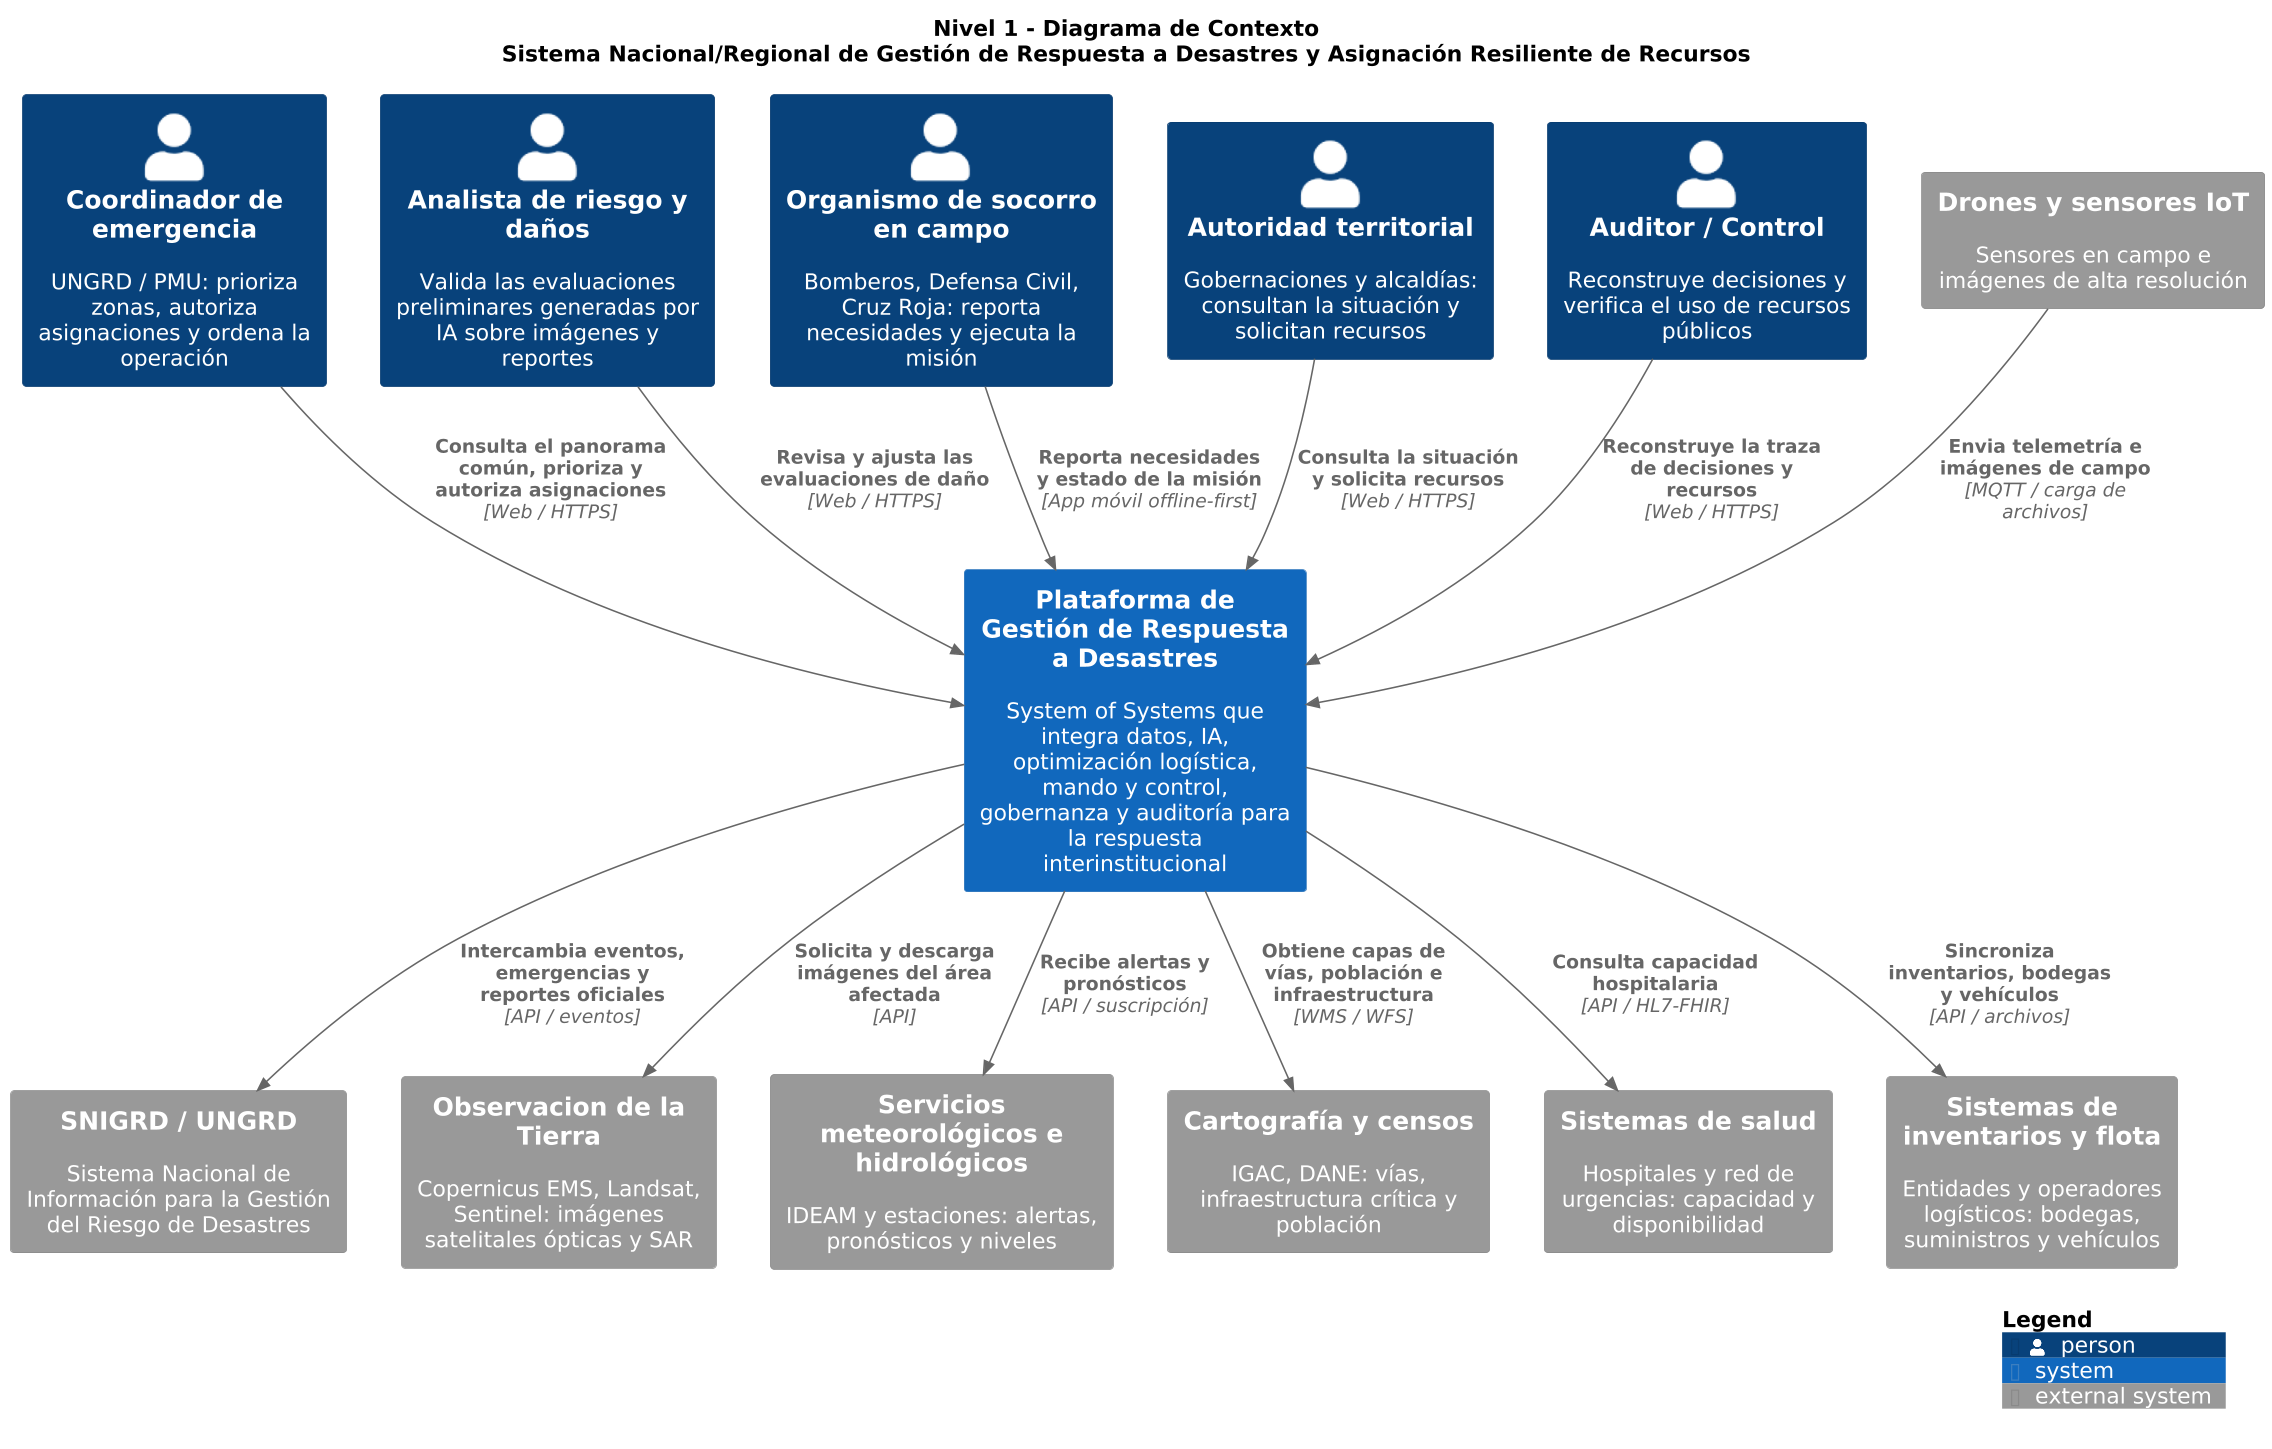
\includegraphics[width=\textwidth]{figuras/c4_l1_contexto.png}
  \caption{Nivel 1 --- Diagrama de contexto del sistema.}
  \label{fig:c4-contexto}
\end{figure}

\subsection{Nivel 2: diagrama de contenedores}

La plataforma se organiza en tres capas de contenedores: presentación y acceso,
servicios y datos. La separación entre el bus de eventos y las bases de datos
permite que la evaluación de daños dispare el recálculo de asignaciones sin
acoplar los servicios entre sí, y que el COP reciba las actualizaciones de
situación en tiempo real.

\begin{landscape}
\begin{figure}[p]
  \centering
  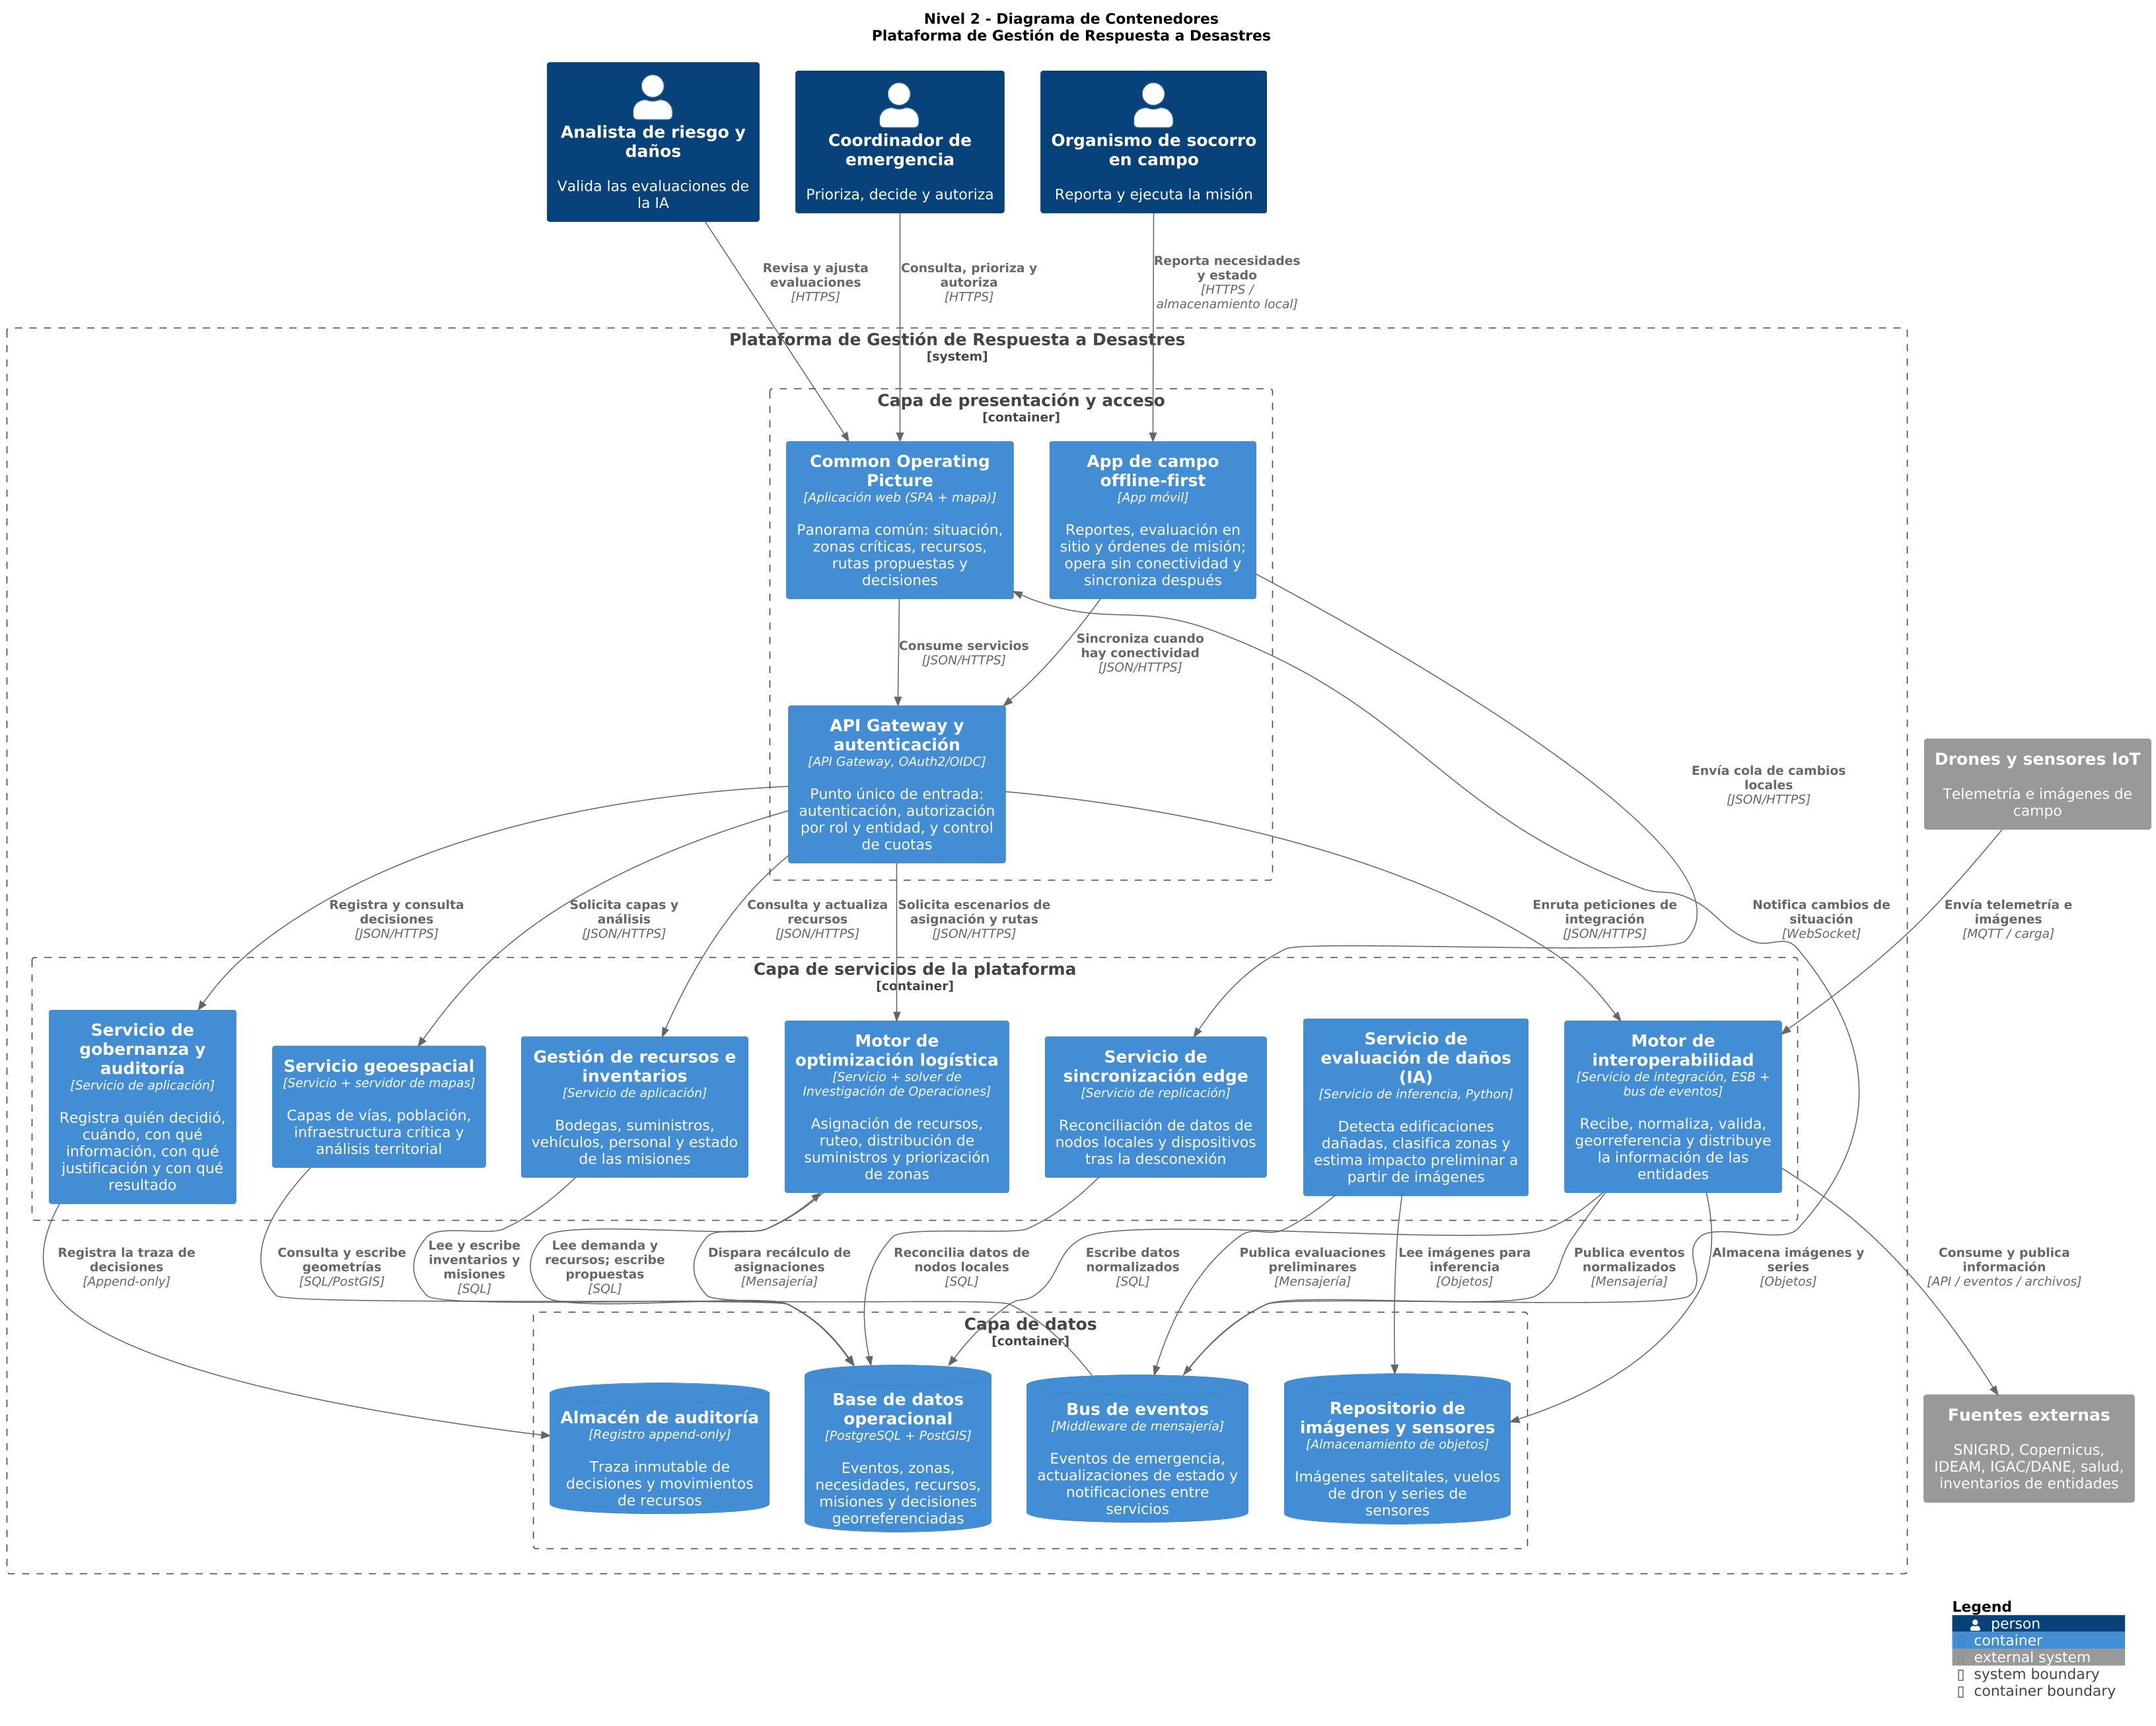
\includegraphics[height=0.92\textheight]{figuras/c4_l2_contenedores.png}
  \caption{Nivel 2 --- Diagrama de contenedores de la plataforma.}
  \label{fig:c4-contenedores}
\end{figure}
\end{landscape}

La tabla~\ref{tab:c4-modulos} muestra la correspondencia entre los módulos
funcionales enunciados en la sección 5.3 y los contenedores del nivel 2, de modo
que la arquitectura de aplicaciones y la vista C4 describan el mismo sistema.

\begin{table}[htbp]
\centering
\caption{Correspondencia entre los módulos de la arquitectura de aplicaciones y
los contenedores C4.}
\label{tab:c4-modulos}
\begin{tabularx}{\textwidth}{@{}LL@{}}
\toprule
\textbf{Módulo (sección 5.3)} & \textbf{Contenedor(es) del nivel 2} \\
\midrule
Motor de interoperabilidad & Motor de interoperabilidad + bus de eventos \\
Sistema GIS y visualización & Servicio geoespacial + Common Operating Picture \\
Módulo de evaluación de daños & Servicio de evaluación de daños (IA) + repositorio de imágenes \\
Módulos de IA y analítica & Servicio de evaluación de daños (IA) \\
Motor de optimización logística & Motor de optimización logística \\
Gestión de inventarios y recursos & Gestión de recursos e inventarios \\
Sistema de mando y coordinación & Common Operating Picture + app de campo offline-first \\
Auditoría, seguridad y administración & API Gateway, servicio de gobernanza y almacén de auditoría \\
\bottomrule
\end{tabularx}
\end{table}

\subsection{Nivel 3: componentes del motor de interoperabilidad}

Este contenedor materializa el flujo \emph{recibir $\rightarrow$ normalizar
$\rightarrow$ validar $\rightarrow$ georreferenciar $\rightarrow$ distribuir} de
la sección 4.2. Dos componentes merecen atención: el catálogo de fuentes y
contratos, que concentra los acuerdos de intercambio con cada entidad, y el
registrador de procedencia, que garantiza el requisito de que cada dato conserve
origen, fecha de actualización y nivel de confianza.

\begin{figure}[p]
  \centering
  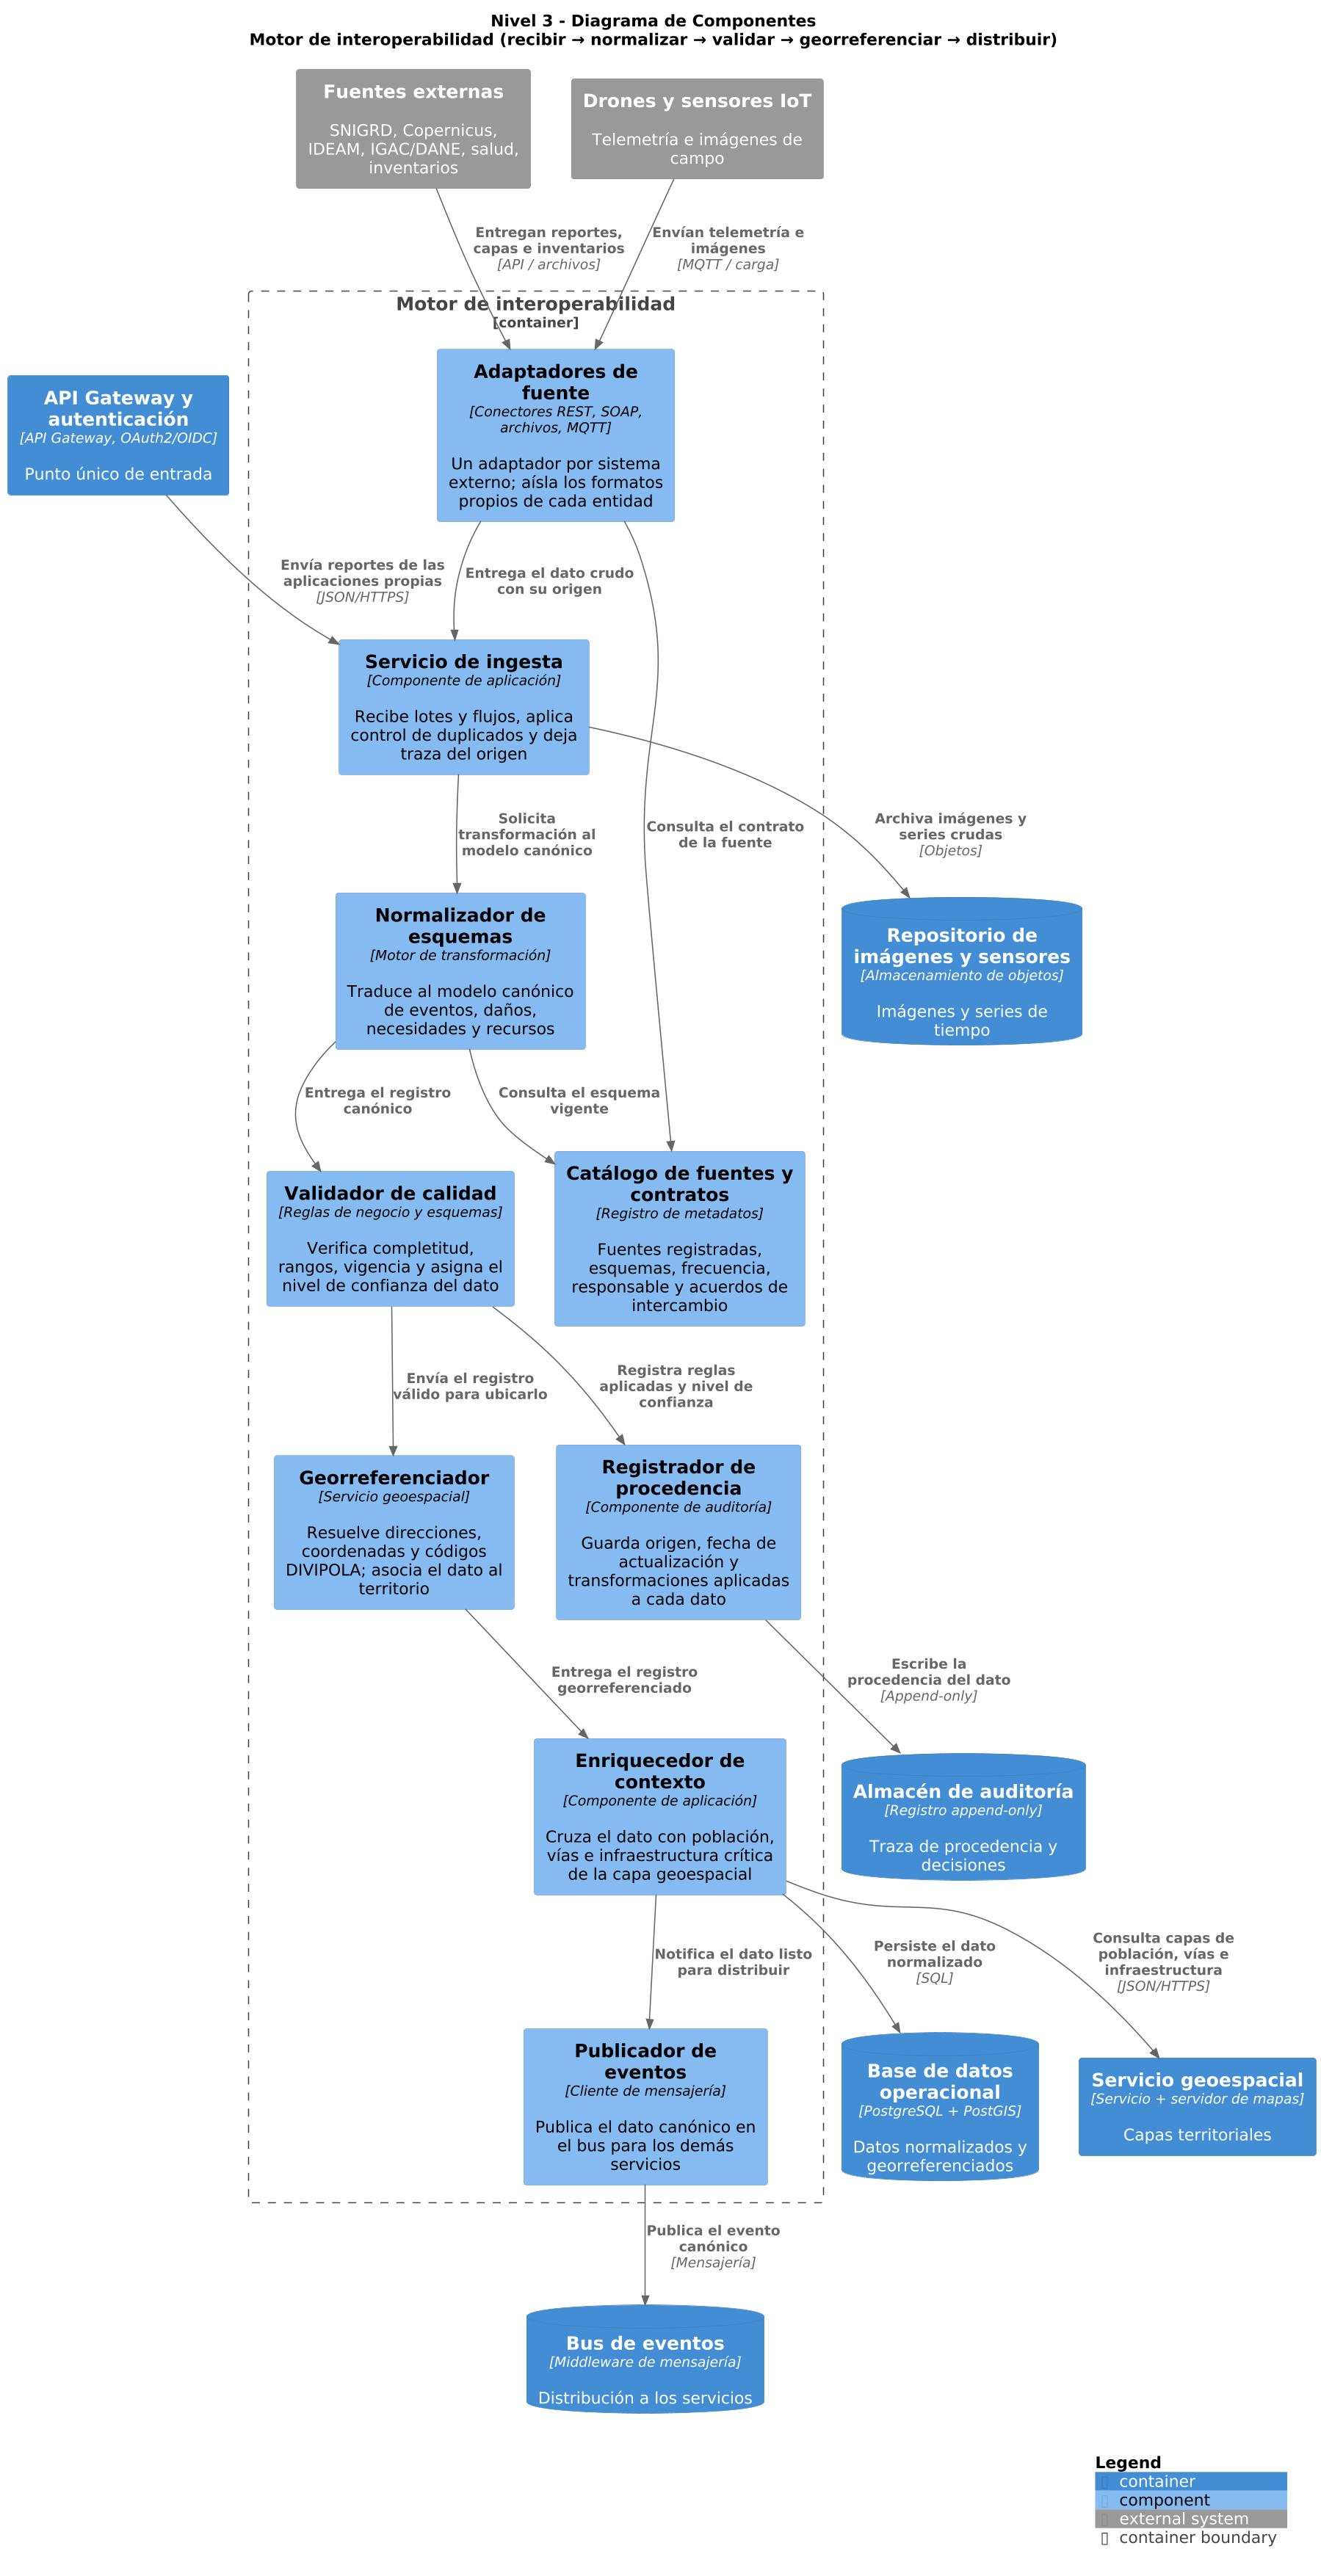
\includegraphics[height=0.88\textheight]{figuras/c4_l3_interoperabilidad.png}
  \caption{Nivel 3 --- Componentes del motor de interoperabilidad.}
  \label{fig:c4-interop}
\end{figure}

\subsection{Nivel 3: componentes del servicio de evaluación de daños}

El diseño hace explícito que la IA no decide. Entre el modelo y el resto del
sistema se interpone una cola de revisión humana: solo las evaluaciones
validadas por el analista se publican en el bus y quedan disponibles para la
optimización. El monitor de desempeño registra precisión, \emph{recall},
F1-score y falsos positivos por tipo de desastre, que son las métricas de la
sección~\ref{sec:metricas}.

\begin{figure}[p]
  \centering
  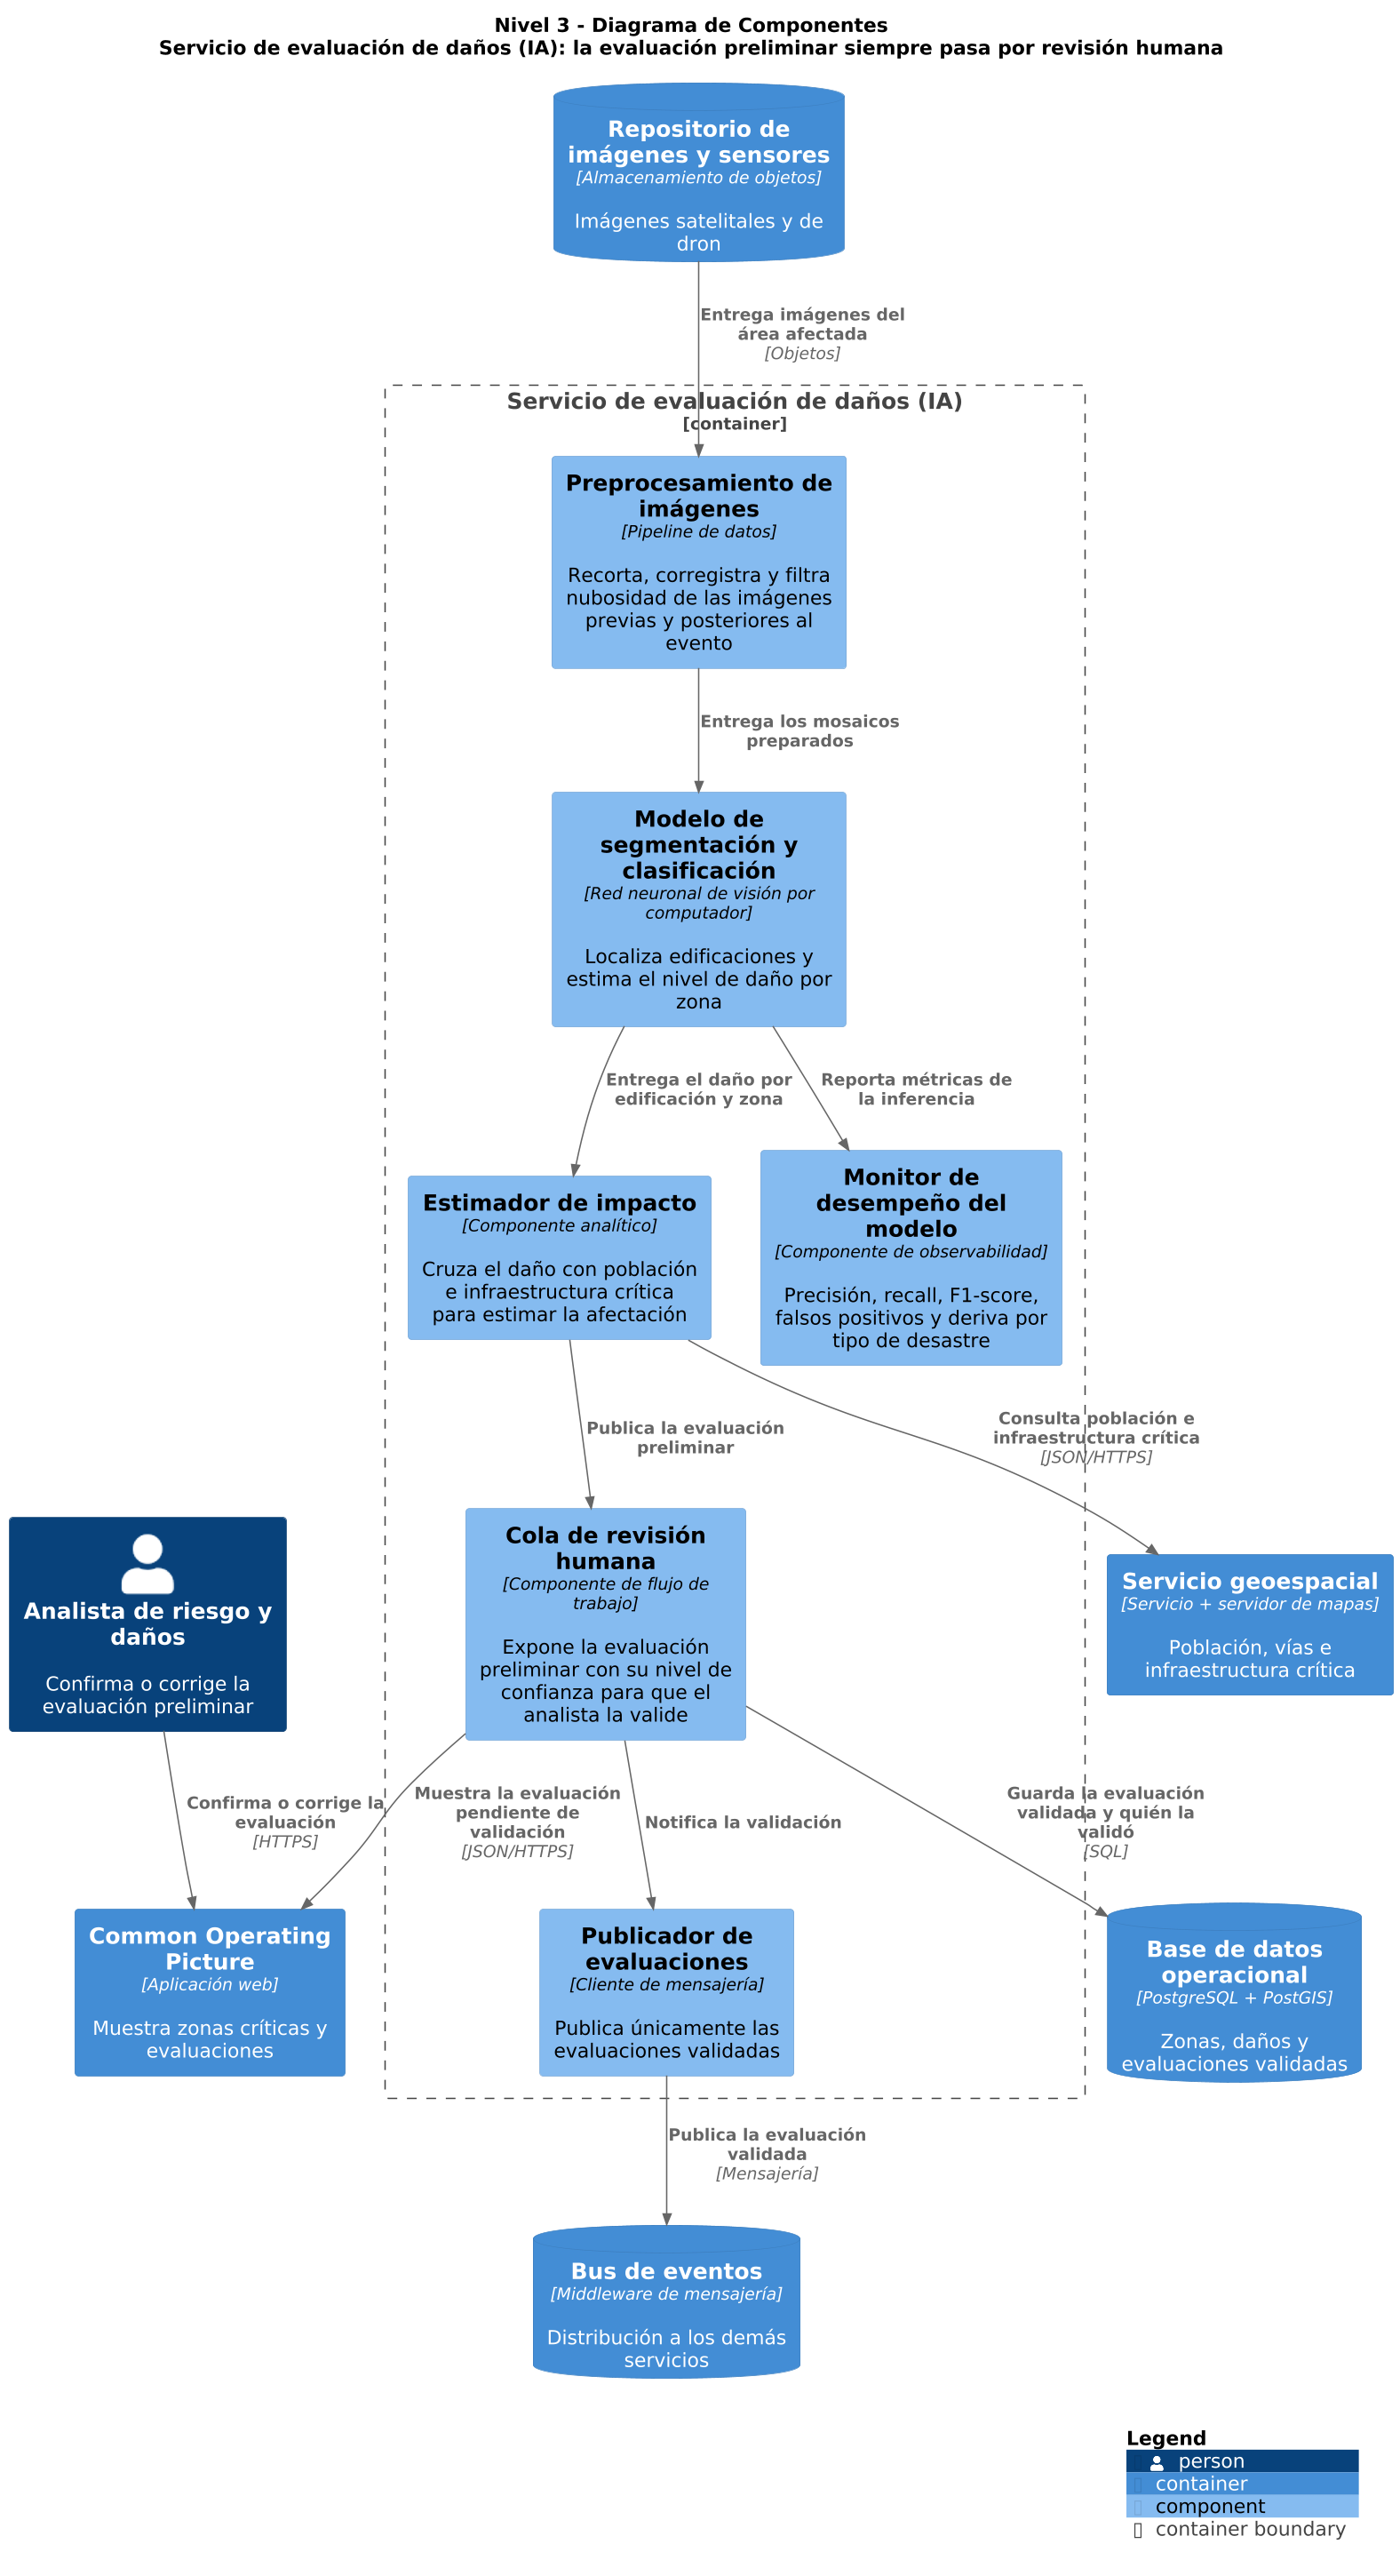
\includegraphics[height=0.88\textheight]{figuras/c4_l3_ia.png}
  \caption{Nivel 3 --- Componentes del servicio de evaluación de daños (IA).}
  \label{fig:c4-ia}
\end{figure}

\subsection{Nivel 3: componentes del motor de optimización logística}

El motor no entrega una orden sino alternativas comparadas. El comparador de
escenarios evalúa cada solución por cobertura, tiempo, kilómetros y costo, y el
explicador expone los supuestos y las restricciones activas, de manera que el
coordinador pueda validar, modificar o rechazar la propuesta con criterio. La
decisión adoptada se registra en el servicio de gobernanza, cerrando la cadena
crítica de la sección 1.

\begin{figure}[p]
  \centering
  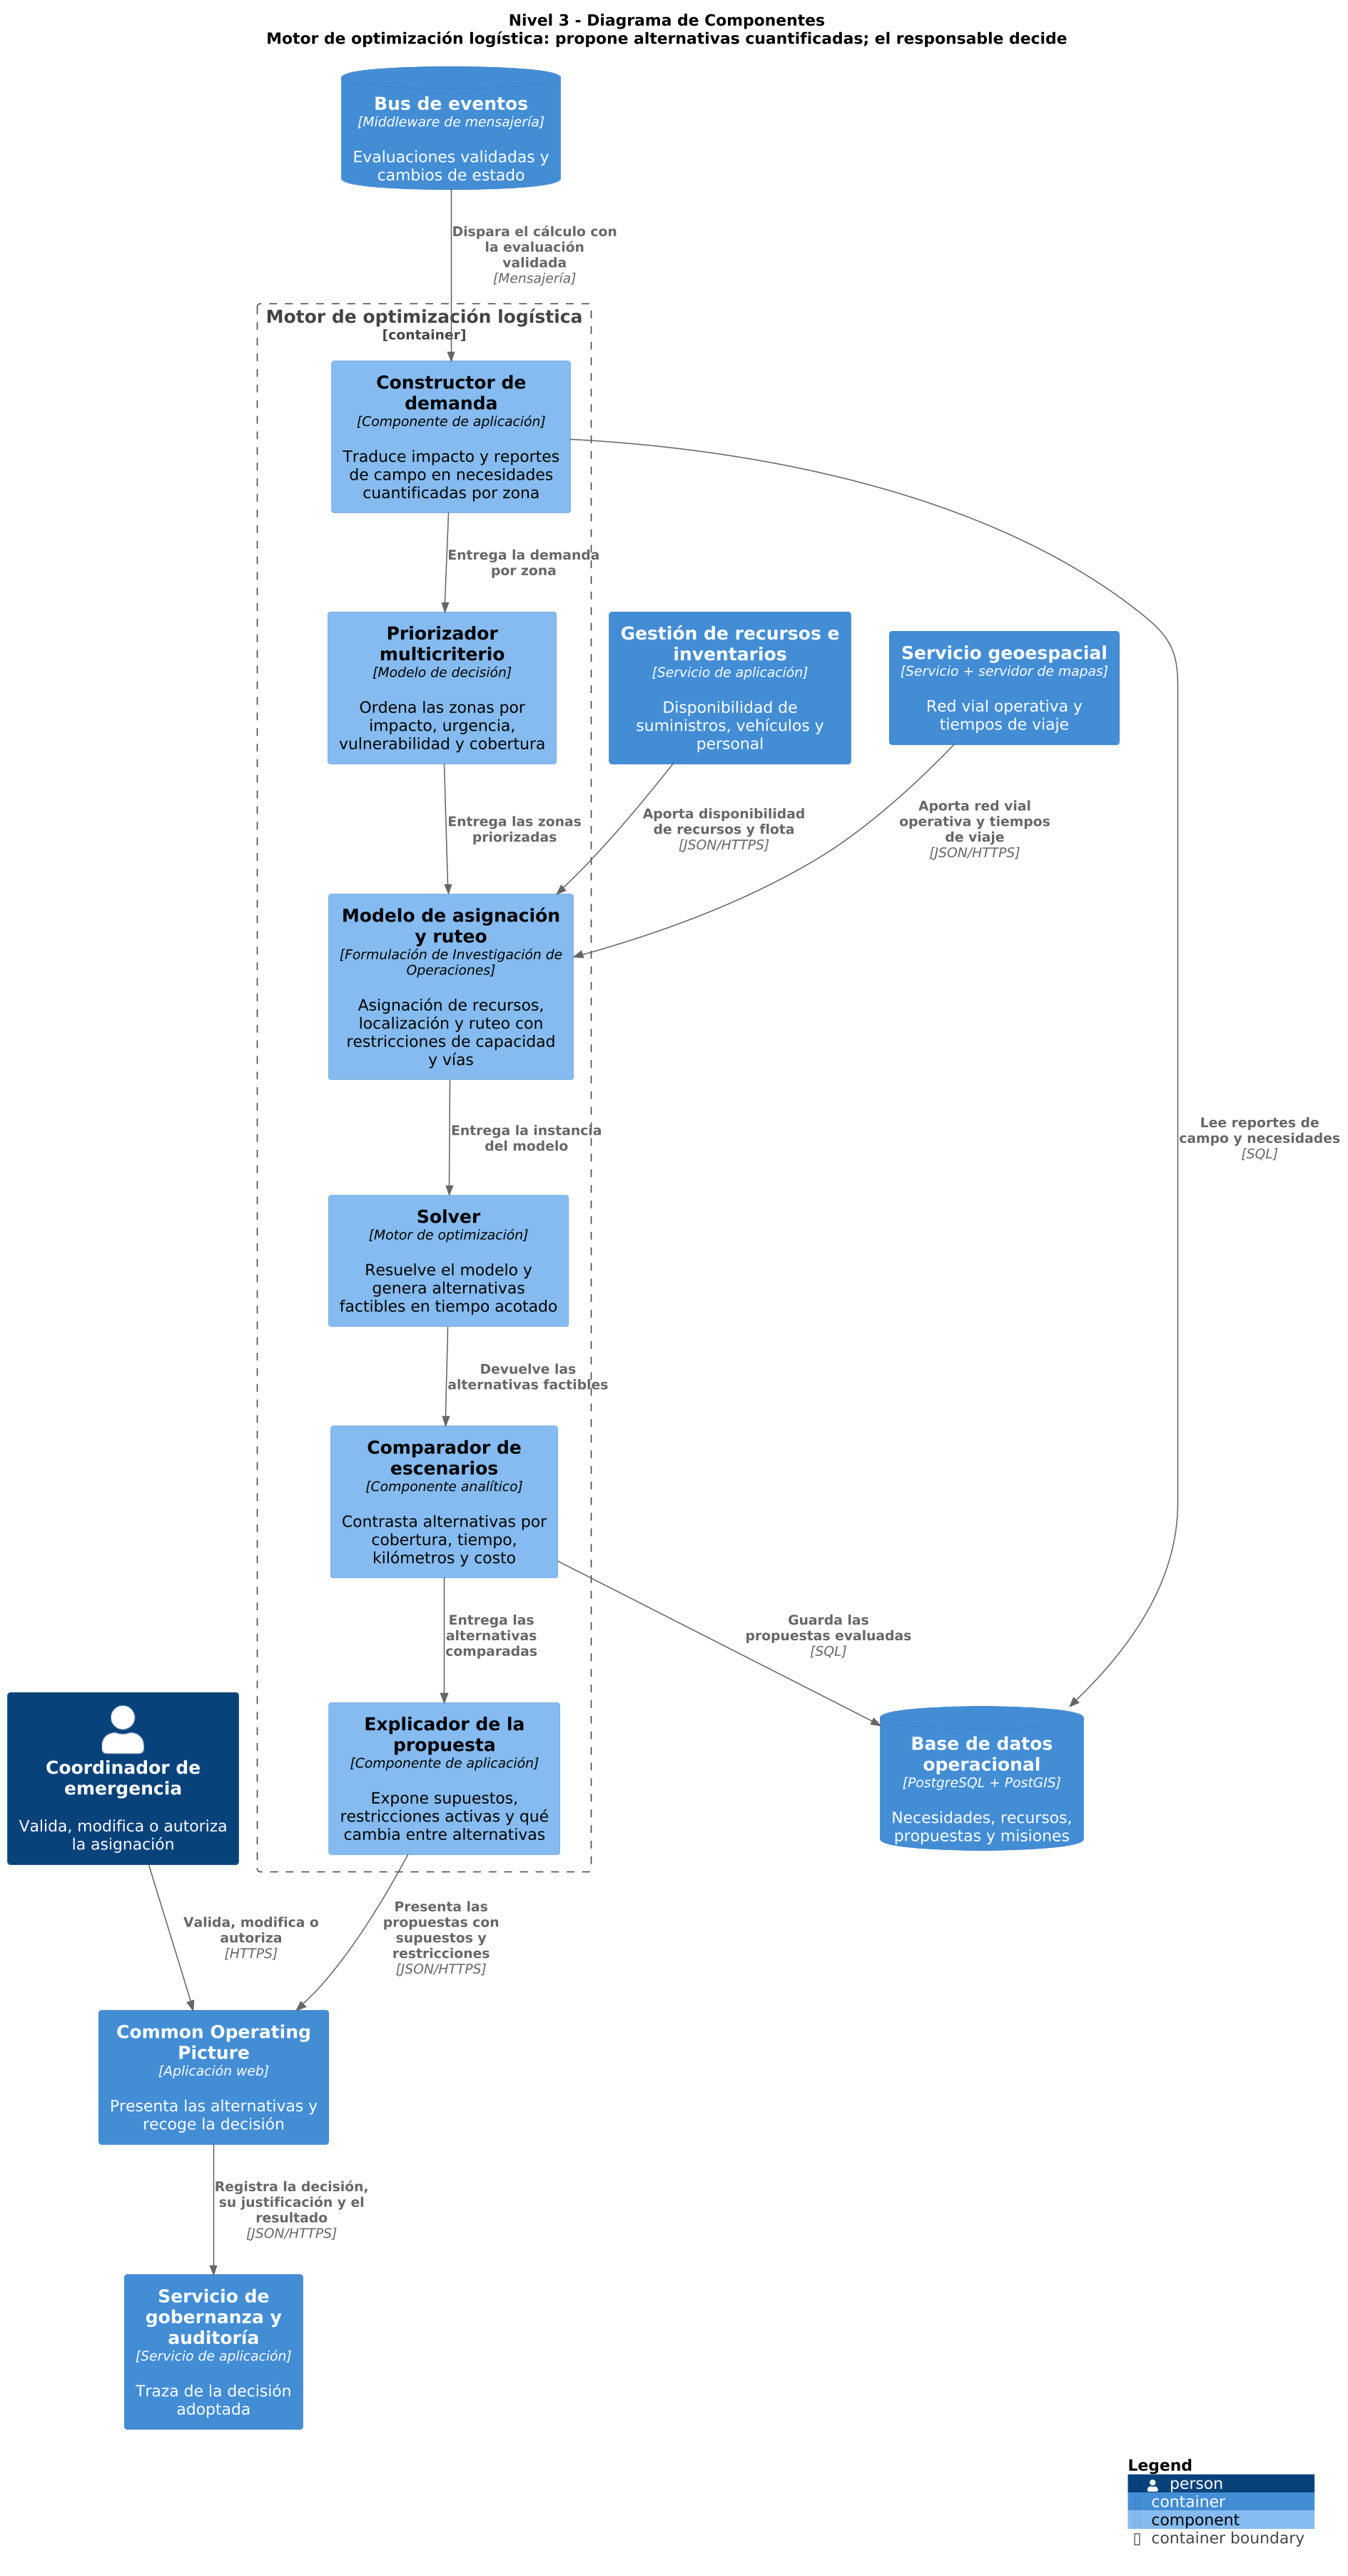
\includegraphics[height=0.88\textheight]{figuras/c4_l3_optimizacion.png}
  \caption{Nivel 3 --- Componentes del motor de optimización logística.}
  \label{fig:c4-opt}
\end{figure}

\subsection{Despliegue y operación resiliente}

El diagrama de despliegue muestra tres ubicaciones: la nube nacional, el nodo
\emph{edge} del puesto de mando unificado municipal y los dispositivos de campo.
El nodo municipal conserva una réplica territorial de la base operacional y un
optimizador acotado, de modo que el municipio pueda seguir coordinando con el
último estado conocido aunque caiga el enlace nacional. El agente de
sincronización encola los cambios locales y los reconcilia al restablecerse la
conexión, que es el mecanismo concreto detrás del indicador de operaciones
sostenidas con conectividad degradada.

\begin{landscape}
\begin{figure}[p]
  \centering
  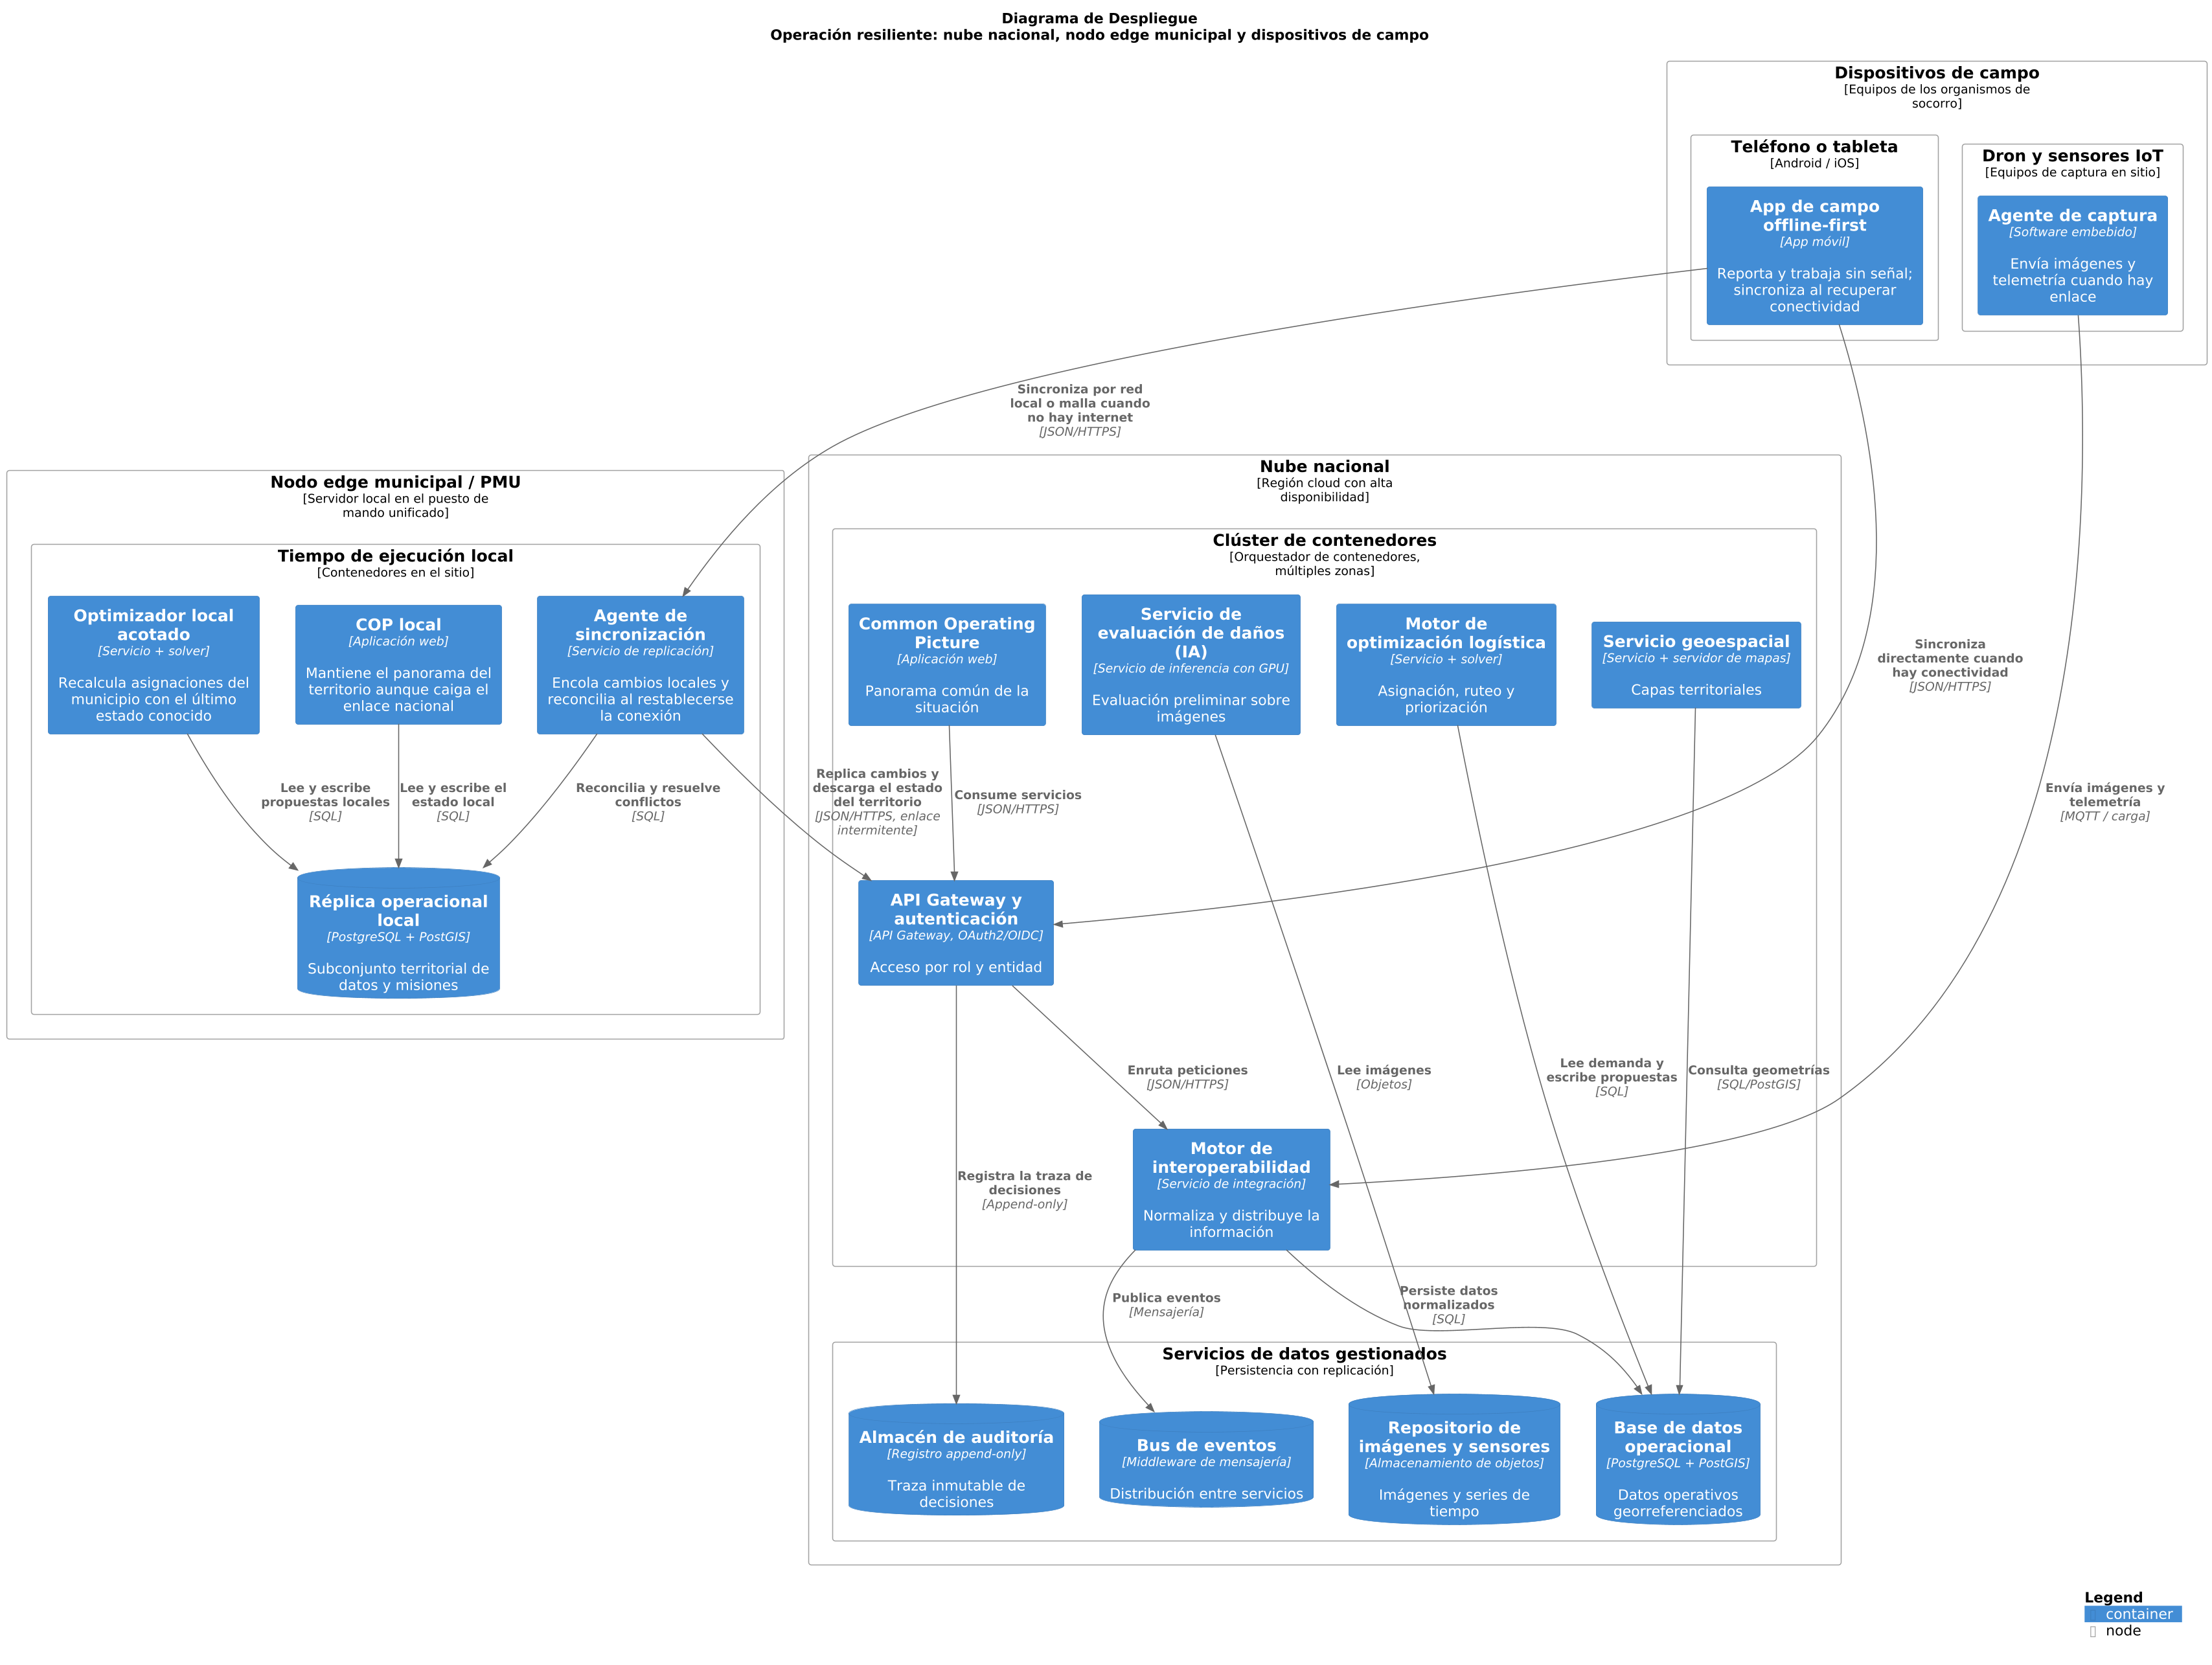
\includegraphics[height=0.92\textheight]{figuras/c4_despliegue.png}
  \caption{Diagrama de despliegue --- nube nacional, nodo \emph{edge} municipal
  y dispositivos de campo.}
  \label{fig:c4-despliegue}
\end{figure}
\end{landscape}

\subsection{Decisiones arquitectónicas}

La tabla~\ref{tab:adr} recoge las decisiones que explican por qué la
arquitectura tiene esta forma y no otra. Cada una responde a una restricción del
problema, no a una preferencia tecnológica.

\begin{table}[htbp]
\centering
\caption{Decisiones arquitectónicas, alternativa descartada y justificación.}
\label{tab:adr}
\begin{tabularx}{\textwidth}{@{}p{3.6cm}LL@{}}
\toprule
\textbf{Decisión} & \textbf{Alternativa descartada} & \textbf{Justificación} \\
\midrule
Integración mediante adaptadores y bus de eventos &
Un sistema único que reemplace los sistemas de cada entidad &
Las entidades conservan sus capacidades; reduce el riesgo y la resistencia
institucional. \\
\addlinespace
Modelo canónico con procedencia y nivel de confianza &
Replicar los datos en el formato propio de cada fuente &
Permite comparar información heterogénea y auditar de dónde salió cada dato. \\
\addlinespace
IA con revisión humana obligatoria &
Evaluación automática publicada directamente &
El desempeño del modelo varía según el desastre y el territorio; evita la caja
negra en decisiones críticas. \\
\addlinespace
Separar predicción, optimización y autorización &
Un único motor que decida de extremo a extremo &
Cada etapa se puede validar y medir por separado; la responsabilidad de la
decisión permanece en la persona. \\
\addlinespace
Nodo \emph{edge} municipal y app \emph{offline-first} &
Dependencia total de la nube nacional &
La conectividad es justamente lo que falla en una emergencia. \\
\addlinespace
Auditoría \emph{append-only} separada de la base operacional &
Registrar la traza en las mismas tablas operativas &
La traza no debe poder alterarse al corregir el estado de la operación. \\
\addlinespace
Optimización con tiempo de cómputo acotado &
Buscar el óptimo global sin límite de tiempo &
En respuesta a desastres una buena alternativa a tiempo vale más que la óptima
tarde. \\
\bottomrule
\end{tabularx}
\end{table}

\subsection{Trazabilidad con la arquitectura empresarial}

La vista C4 no sustituye a la arquitectura empresarial de la sección 5: la hace
verificable. La tabla~\ref{tab:c4-ae} muestra cómo cada capa se materializa en
elementos concretos del modelo.

\begin{table}[htbp]
\centering
\caption{Trazabilidad entre las capas de arquitectura empresarial y la vista C4.}
\label{tab:c4-ae}
\begin{tabularx}{\textwidth}{@{}p{3.6cm}L@{}}
\toprule
\textbf{Capa} & \textbf{Elementos C4 que la materializan} \\
\midrule
Negocio & Actores y sistemas externos del nivel 1; puntos de decisión humana en
los niveles 3 (cola de revisión y autorización de la asignación). \\
\addlinespace
Información & Modelo canónico del motor de interoperabilidad; base de datos
operacional, repositorio de imágenes y almacén de auditoría del nivel 2. \\
\addlinespace
Aplicaciones & Contenedores de la capa de servicios y sus componentes
documentados en el nivel 3. \\
\addlinespace
Tecnología & Diagrama de despliegue: nube nacional, nodo \emph{edge} municipal y
dispositivos de campo. \\
\bottomrule
\end{tabularx}
\end{table}

% =====================================================================
\section{Prototipo: nodo \emph{edge} de alertas en tiempo real con conectividad intermitente}
\label{sec:prototipo}
% =====================================================================

La arquitectura de las secciones anteriores es deliberadamente amplia. Esta
sección delimita la parte que se implementa y se mide. El criterio de selección
fue elegir el problema tecnológico más crítico para que el resto de la
arquitectura funcione en una emergencia real: que la detección y las alertas no
dependan de un enlace que, en un desastre, es justamente lo primero que falla.

\subsection{Problema tecnológico y pregunta del prototipo}

En el diseño actual, las fuentes de campo (sensores IoT, drones) alimentan al
motor de interoperabilidad en la nube nacional. Si la detección de eventos
ocurre solo en la nube, cada alerta paga el viaje de ida y vuelta por la red
de área amplia (WAN) y, cuando el enlace cae, el municipio queda sin alertas y
los datos producidos durante la caída se pierden. El diagrama de despliegue
(figura~\ref{fig:c4-despliegue}) ya plantea un nodo \emph{edge} en el puesto de
mando unificado (PMU) con réplica local y agente de sincronización. El
prototipo construye ese nodo y lo somete a una caída controlada del enlace.

\begin{quote}
\itshape
¿Puede un nodo \emph{edge} municipal mantener la detección y la emisión de
alertas en tiempo real durante una caída del enlace con la nube, sin perder
lecturas, y converger con el nivel central al reconectarse sin generar
duplicados ni romper la trazabilidad?
\end{quote}

La pregunta se descompone en cinco hipótesis verificables:

\begin{enumerate}[leftmargin=*,label=\textbf{H\arabic*.}]
  \item La latencia de alerta en el \emph{edge} se mantiene por debajo de
        1\,s (p95), también durante la caída; la línea base solo nube paga la
        latencia de la WAN y pierde las alertas durante la caída.
  \item Ninguna lectura se pierde: tras la reconexión, la nube contiene
        exactamente el conjunto de lecturas producidas en campo.
  \item Los reenvíos causados por confirmaciones (ACK) perdidas no generan
        duplicados en la nube.
  \item El \emph{backlog} acumulado en el \emph{edge} se vacía en un tiempo
        acotado después de la reconexión.
  \item La bitácora de auditoría permanece íntegra y detecta cualquier
        alteración de un registro pasado.
\end{enumerate}

\subsection{Alcance: qué se construye y qué se simula}

La tabla~\ref{tab:alcance} responde la pregunta central de esta entrega. El
criterio es construir de verdad todo lo que está en la ruta crítica de la
hipótesis y simular lo que solo aporta datos o contexto. Los protocolos son
reales aunque el hardware sea simulado: los dispositivos publican por MQTT y la
sincronización viaja por HTTP a través de un enlace con latencia y cortes.

\begin{table}[htbp]
\centering
\caption{Delimitación del prototipo: componentes construidos, simulados y fuera de alcance.}
\label{tab:alcance}
\small
\begin{tabularx}{\textwidth}{@{}p{3.6cm}p{2.4cm}L@{}}
\toprule
\textbf{Elemento} & \textbf{Tratamiento} & \textbf{Detalle} \\
\midrule
\multicolumn{3}{@{}l}{\textit{Nodo edge del PMU (contenedores del diagrama de despliegue)}} \\
Broker MQTT & Construido & Mosquitto, QoS~1; recibe la telemetría de campo por la red local. \\
Ingesta y validación & Construido & Valida cada mensaje contra el contrato \texttt{Telemetry} y descarta reentregas por \texttt{event\_id}. \\
Detector de eventos & Construido & Umbrales por tipo de sensor y z-score móvil por dispositivo; enfriamiento de 10\,s para no repetir alertas del mismo episodio. \\
Almacén local con \emph{outbox} & Construido & SQLite en modo WAL; lectura y alerta se guardan en una sola transacción antes de cualquier envío. Materializa la réplica operacional local. \\
Agente de sincronización & Construido & Lotes de hasta 500 lecturas; marca como sincronizado solo con ACK; reintento con \emph{backoff} exponencial (0,5 a 8\,s). \\
Bitácora de auditoría & Construido & \emph{Append-only} encadenada con SHA-256: alertas, lotes sincronizados y cambios de estado del enlace. \\
COP local & Construido (mínimo) & Tablero web con alertas en vivo (\emph{Server-Sent Events}), estado del enlace y del \emph{backlog}. \\
\addlinespace
\multicolumn{3}{@{}l}{\textit{Nube nacional}} \\
API central & Construida (mínima) & Receptor idempotente de lotes (\texttt{POST /api/v1/sync}) y, para la línea base, ingesta directa con detección en la nube (\texttt{POST /api/v1/ingest}). \\
Base consolidada & Construida (mínima) & SQLite con \texttt{event\_id} como llave primaria. En producción sería la base operacional PostgreSQL/PostGIS. \\
\addlinespace
\multicolumn{3}{@{}l}{\textit{Entorno}} \\
Sensores y drones & Simulados & 50 dispositivos a 1\,Hz: 20 limnímetros, 15 pluviómetros, 10 acelerómetros y 5 drones con conteo de personas (el clasificador a bordo se simula). \\
Enlace WAN & Emulado & Proxy TCP propio: 200\,$\pm$\,80\,ms por sentido y corte controlado (cierra conexiones abiertas y rechaza nuevas). \\
Pérdida de ACK & Inyectada & La nube confirma la escritura pero responde 503 con probabilidad 0,1, para forzar reenvíos. \\
Respondientes locales & Simulados & Suscriptor MQTT que registra la hora de llegada de cada alerta. \\
\addlinespace
\multicolumn{3}{@{}l}{\textit{Fuera del prototipo}} \\
Optimización logística, IA sobre imágenes, GIS, interoperabilidad con SNIGRD/UNGRD, app de campo, autenticación & No se construyen & Siguen descritos en la arquitectura general; el prototipo no depende de ellos para responder la pregunta. \\
\bottomrule
\end{tabularx}
\end{table}

\subsection{Arquitectura del prototipo}

La figura~\ref{fig:prototipo} muestra los contenedores del prototipo con el
mismo nivel de detalle del nivel~2 de C4 (figura~\ref{fig:c4-contenedores}):
en azul lo construido, en gris discontinuo lo simulado o emulado. Los números indican el flujo
principal. El prototipo corresponde a tres contenedores del diagrama de
despliegue: COP local, agente de sincronización y réplica operacional local.
Agrega dos que el diseño general dejaba implícitos dentro del agente de
captura y del motor de interoperabilidad: el broker MQTT local y el detector de
eventos en el borde.

Los dos servicios construidos, el nodo \emph{edge} y la API de la nube, están
implementados en Java~21 con Spring Boot~3.5, como un proyecto Maven
multimódulo: un módulo compartido con los contratos y el detector, y un módulo
por servicio. El nodo \emph{edge} usa Eclipse Paho como cliente MQTT, SQLite
mediante Spring JDBC para el almacén local y \emph{Server-Sent Events} para el
COP; la nube expone su API con Spring MVC y la documenta con OpenAPI. Las
herramientas de prueba (simulador de dispositivos, emulador del enlace y
experimento) están en Python y solo hablan con los servicios a través de sus
contratos: MQTT, HTTP/JSON y el archivo SQLite del nodo \emph{edge}, que el
experimento lee para verificar la auditoría.

\begin{figure}[p]
  \centering
  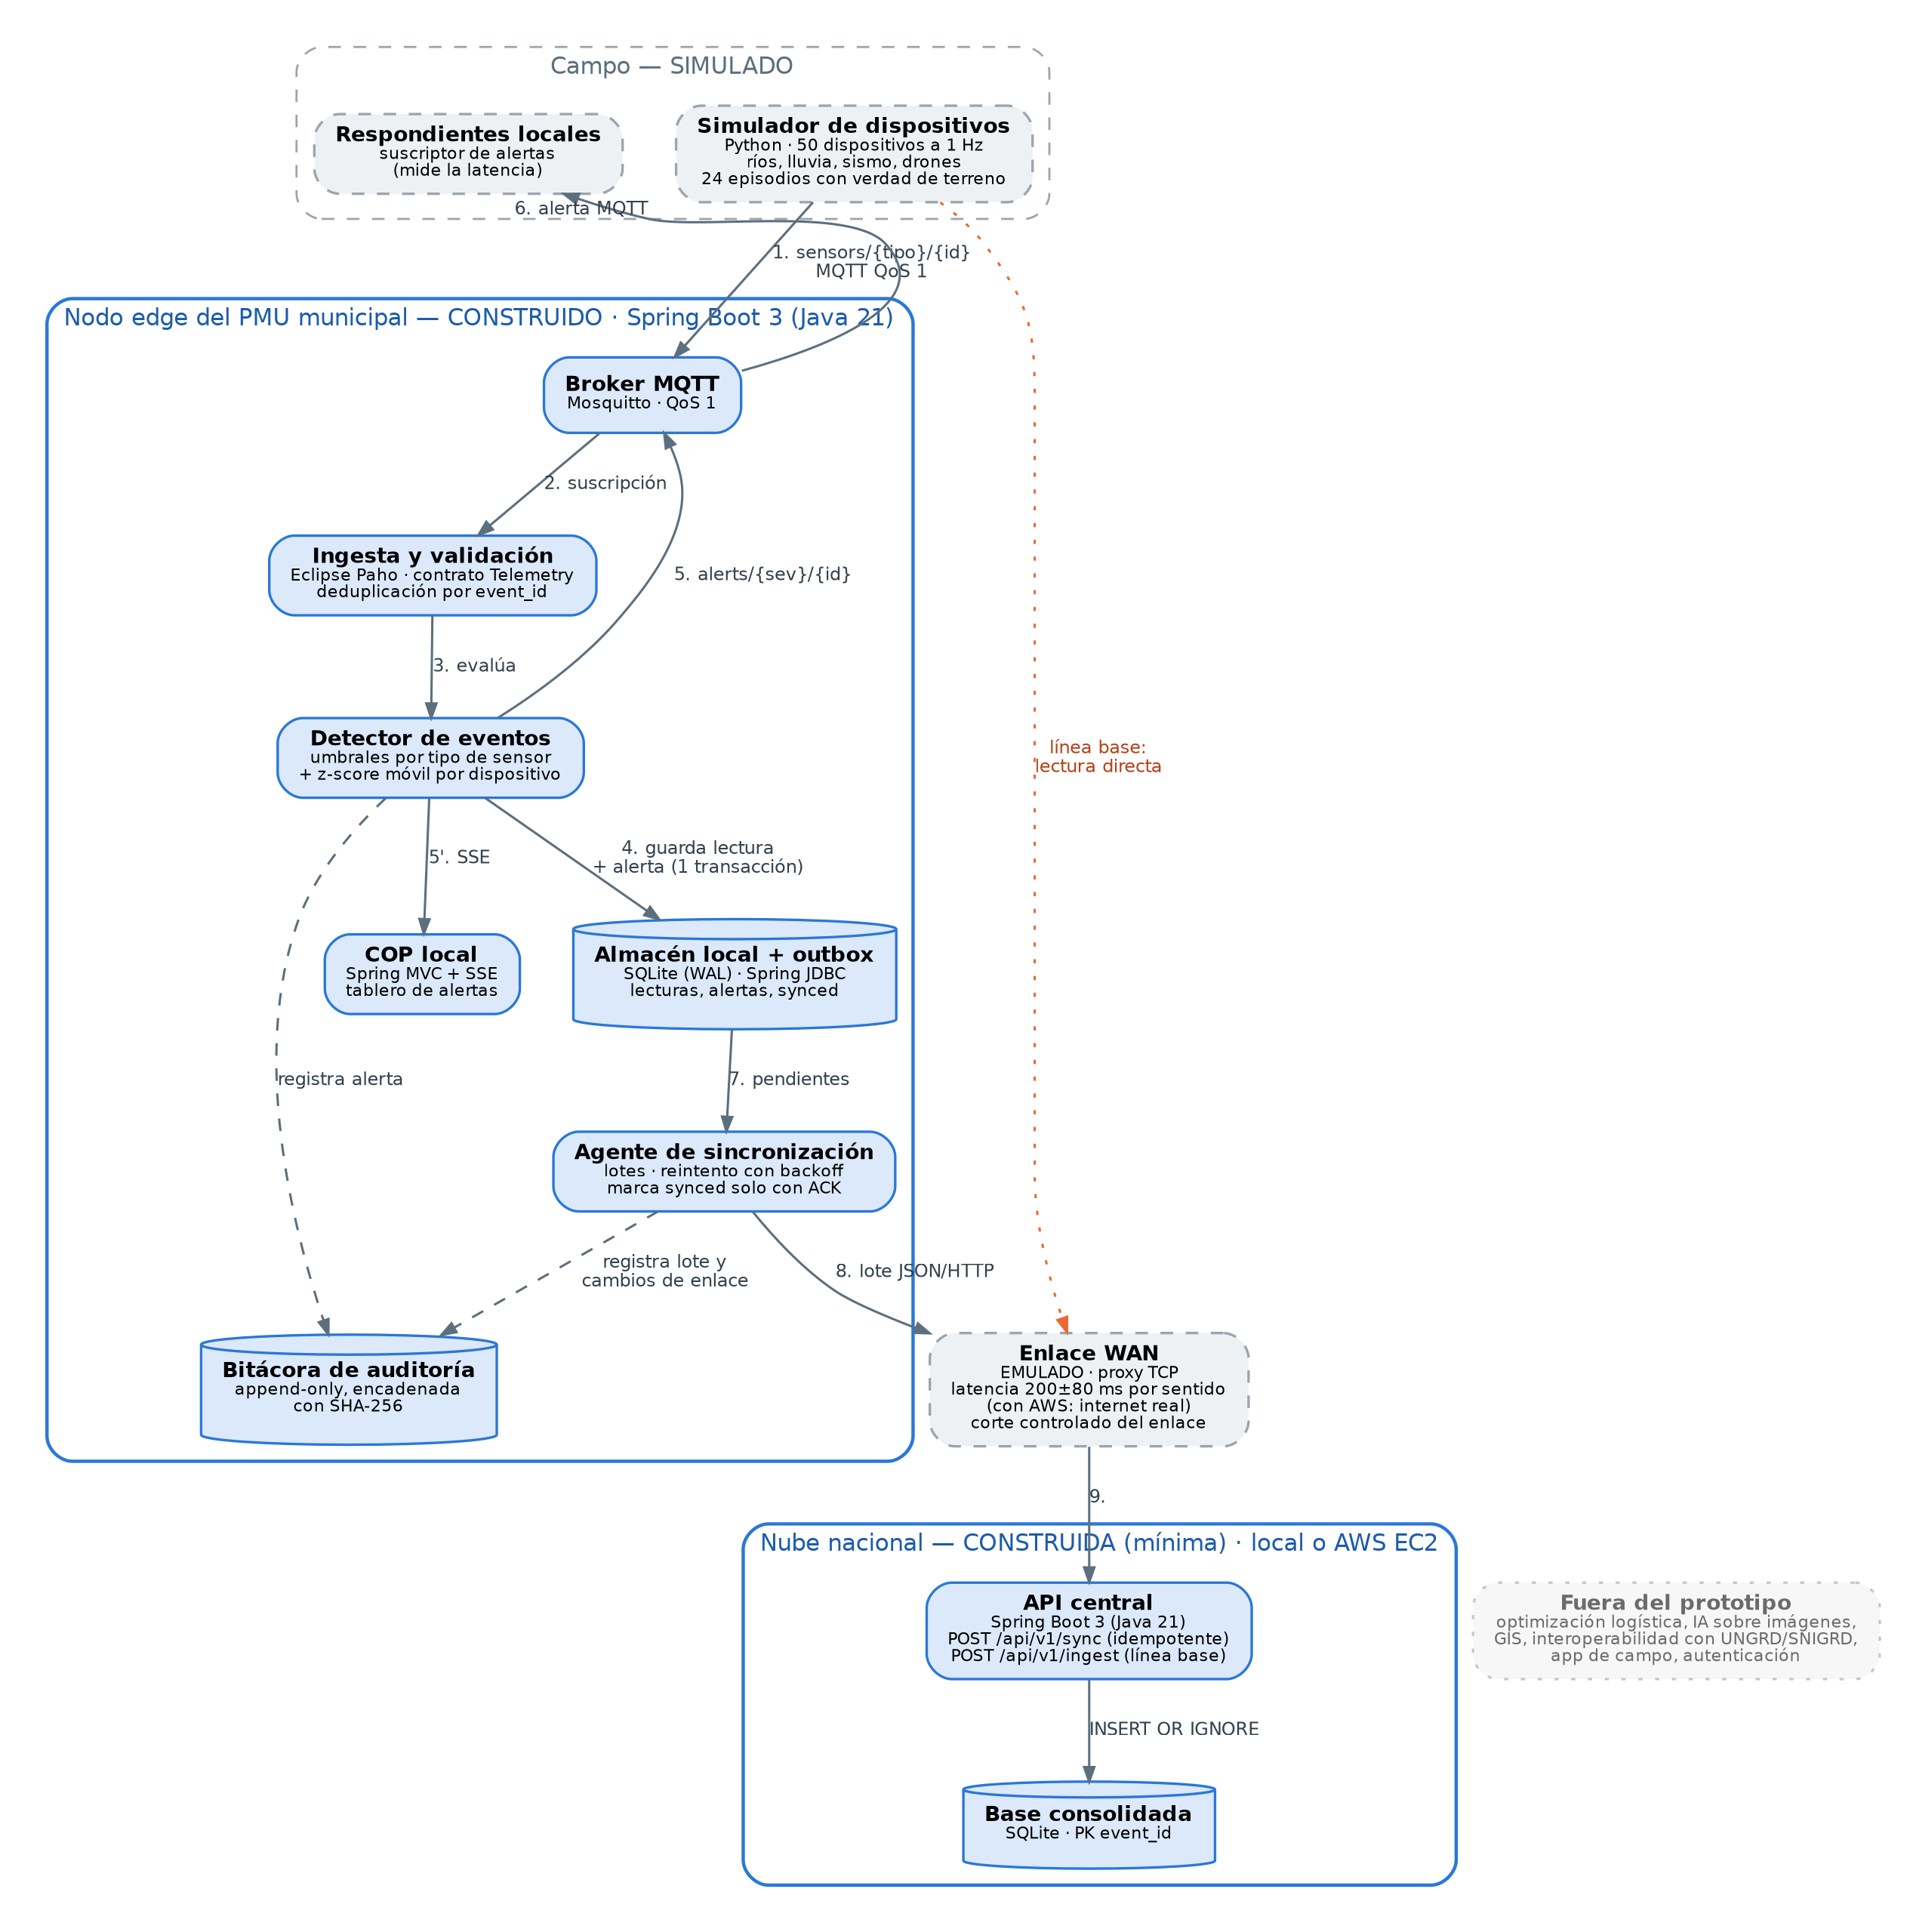
\includegraphics[width=\textwidth,height=0.86\textheight,keepaspectratio]{figuras/prototipo_contenedores.png}
  \caption{Contenedores del prototipo. Azul: construido. Gris discontinuo:
  simulado o emulado. Naranja punteado: ruta de la línea base solo nube.}
  \label{fig:prototipo}
\end{figure}

\subsection{Contratos}

Todos los mensajes que cruzan un límite de proceso tienen un contrato
explícito, versionado en el repositorio (\texttt{contracts/}) como JSON Schema
y OpenAPI, y validado en tiempo de ejecución. El \texttt{event\_id} (UUID
generado en el dispositivo) es la clave de idempotencia de extremo a extremo:
permite deduplicar en el \emph{edge} (reentregas QoS~1) y en la nube
(reenvíos de lotes).

\begin{table}[htbp]
\centering
\caption{Contratos implementados.}
\label{tab:contratos}
\small
\begin{tabularx}{\textwidth}{@{}p{3.1cm}p{3.6cm}L@{}}
\toprule
\textbf{Contrato} & \textbf{Canal} & \textbf{Campos clave y garantía} \\
\midrule
\texttt{Telemetry} & MQTT \texttt{sensors/\{tipo\}/\{id\}}, QoS~1 &
\texttt{event\_id}, \texttt{device\_id}, \texttt{sensor\_type}, \texttt{value},
\texttt{unit}, \texttt{lat}, \texttt{lon}, \texttt{seq}, \texttt{ts\_ms}.
Al menos una vez. \\
\addlinespace
\texttt{Alert} & MQTT \texttt{alerts/\{sev\}/\{id\}}, QoS~1, y SSE &
\texttt{alert\_id}, \texttt{event\_id}, \texttt{severity}, \texttt{rule},
\texttt{score}, \texttt{ts\_event\_ms}, \texttt{ts\_alert\_ms},
\texttt{source}. \\
\addlinespace
\texttt{SyncBatch} / \texttt{SyncAck} & HTTP \texttt{POST /api/v1/sync} &
Lote de lecturas y alertas; la respuesta informa aceptados y duplicados.
Idempotente: reenviar un lote no cambia el estado de la nube. \\
\addlinespace
\texttt{IngestResponse} & HTTP \texttt{POST /api/v1/ingest} &
Solo para la línea base: el dispositivo envía la lectura y recibe la alerta en
la respuesta. \\
\bottomrule
\end{tabularx}
\end{table}

\subsection{Datos}

No se usan datos reales de sensores. El simulador genera un escenario
reproducible (semilla fija) alrededor de coordenadas plausibles de un
municipio de Putumayo. Sobre el ruido normal de cada dispositivo se plantan 24
episodios anómalos de 6\,s, en dispositivos distintos y repartidos a lo largo
de la ejecución, de modo que 12 caen dentro de la ventana de caída: cinco
desbordamientos de río (sobre el umbral crítico), cinco crecidas súbitas que
no alcanzan el umbral y solo detecta el z-score, cinco lluvias intensas, cinco
movimientos sísmicos y cuatro detecciones de personas por dron. El simulador
registra la primera lectura anómala de cada episodio como verdad de terreno,
lo que permite medir de forma objetiva la latencia, la sensibilidad
(\emph{recall}) y la precisión de las alertas.

\subsection{Flujos}

\begin{enumerate}[leftmargin=*]
  \item \textbf{Operación normal.} Dispositivo $\rightarrow$ broker
        $\rightarrow$ ingesta $\rightarrow$ detector $\rightarrow$ almacén
        local (lectura y alerta en una transacción) $\rightarrow$ alerta por
        MQTT y SSE a los respondientes y al COP local. En paralelo, el agente
        de sincronización envía los pendientes a la nube cada 0,5\,s.
  \item \textbf{Caída del enlace.} El agente detecta el error, registra
        \texttt{link\_down} en la auditoría y entra en \emph{backoff}. La
        detección y las alertas continúan sin cambios porque no dependen de la
        nube; las lecturas se acumulan como pendientes en el almacén local.
  \item \textbf{Reconexión.} El siguiente reintento tiene éxito, se registra
        \texttt{link\_up} y el agente vacía el \emph{backlog} en lotes
        consecutivos sin espera.
  \item \textbf{ACK perdido.} La nube guarda el lote pero la confirmación no
        llega. El \emph{edge} no marca las filas y las reenvía; la nube las
        reconoce como duplicadas por llave primaria y no las vuelve a guardar.
  \item \textbf{Línea base solo nube.} Cada dispositivo envía su lectura a la
        nube por la WAN; la nube detecta y devuelve la alerta. Durante la caída
        los envíos fallan y no hay alerta.
\end{enumerate}

\subsection{Decisiones de diseño del prototipo}

\begin{table}[htbp]
\centering
\caption{Decisiones del prototipo, alternativa descartada y justificación.}
\label{tab:adr-prototipo}
\small
\begin{tabularx}{\textwidth}{@{}p{3.6cm}LL@{}}
\toprule
\textbf{Decisión} & \textbf{Alternativa descartada} & \textbf{Justificación} \\
\midrule
MQTT con QoS~1 entre campo y \emph{edge} & HTTP por lectura & Protocolo
estándar de IoT, liviano para enlaces de radio; QoS~1 asegura entrega a cambio
de posibles duplicados, que se resuelven por \texttt{event\_id}. \\
\addlinespace
Patrón \emph{outbox} en SQLite & Enviar directo a la nube y guardar después &
Si el envío falla, el dato ya está persistido; la caída solo hace crecer el
\emph{backlog}. \\
\addlinespace
Receptor idempotente en la nube & Garantizar entrega exactamente una vez en el
transporte & \emph{Exactly-once} en red no es alcanzable; \emph{al menos una
vez} más idempotencia da el mismo efecto observable con un mecanismo simple. \\
\addlinespace
Detección por reglas y z-score & Modelo de aprendizaje profundo en el borde &
Explicable, sin entrenamiento y con costo de cómputo despreciable; un modelo
entrenado es trabajo futuro y se integraría en el mismo punto. \\
\addlinespace
\emph{Backoff} exponencial con tope de 8\,s & Reintento constante e inmediato &
Evita saturar un enlace degradado; el costo es una demora de hasta 8\,s en
notar la reconexión (se mide en H4). \\
\addlinespace
Auditoría encadenada con \emph{hash} & Tabla de registro sin protección &
Cualquier alteración de un registro pasado rompe la cadena desde ese punto y
queda localizada. \\
\bottomrule
\end{tabularx}
\end{table}

\subsection{Diseño experimental}

Se ejecuta el mismo escenario de 120\,s (6\,000 lecturas) dos veces sobre la
misma infraestructura: una con el nodo \emph{edge} y otra con la línea base
solo nube. En ambas, el enlace WAN cae entre los segundos 40 y 80. En la
ejecución \emph{edge} se inyecta además la pérdida del 10\,\% de los ACK. La
latencia de alerta se mide como el tiempo entre la primera lectura anómala de
un episodio y la llegada de su primera alerta al lado de los respondientes
locales. Un episodio cuenta como detectado si al menos una de sus lecturas
genera alerta. Una alerta es verdadera si su lectura pertenece a algún
episodio. Al final se comparan los identificadores de lecturas producidas con
los almacenados en la nube.

Como prueba complementaria de capacidad, se ejecuta el \emph{edge} sin caída
con 500 dispositivos simulados a 10\,Hz (500 mensajes por segundo durante
40\,s). Para H5 se copia la base local, se altera una entrada intermedia de la
bitácora y se verifica la cadena.

El entorno de medición fue un único equipo Windows~11 con Docker Desktop:
nodo \emph{edge} y nube en Spring Boot~3.5 sobre Java~21, broker Mosquitto~2 y
herramientas de prueba en Python~3.13, todos en contenedores. La WAN emulada es
la única fuente de latencia de red.

\subsection{Resultados}

La tabla~\ref{tab:resultados} resume las métricas y las
figuras~\ref{fig:latencia} y~\ref{fig:timeline} muestran su comportamiento.

\begin{table}[htbp]
\centering
\caption{Resultados del experimento: mismo escenario, caída de 40\,s del enlace.}
\label{tab:resultados}
\small
\begin{tabularx}{\textwidth}{@{}Lrr@{}}
\toprule
\textbf{Métrica} & \textbf{Solo nube} & \textbf{Edge} \\
\midrule
Lecturas generadas & 6\,000 & 6\,000 \\
Lecturas perdidas & 2\,012 (33.5 \%) & 0 (0.0 \%) \\
Episodios detectados (recall) & 14/24 (0.58) & 24/24 (1.00) \\
Episodios detectados durante la caída & 2/12 & 12/12 \\
Precisión de las alertas & 1.00 & 1.00 \\
Latencia de alerta p50 (ms) & 448 & 2 \\
Latencia de alerta p95 (ms) & 2\,379 & 23 \\
Duplicados almacenados en la nube & 0 & 0 \\
Reenvíos rechazados por idempotencia & -- & 263 \\
Backlog máximo en edge (lecturas) & -- & 2\,448 \\
Vaciado del backlog tras reconectar (s) & -- & 9.8 \\
\bottomrule
\end{tabularx}

\end{table}

\begin{figure}[htbp]
  \centering
  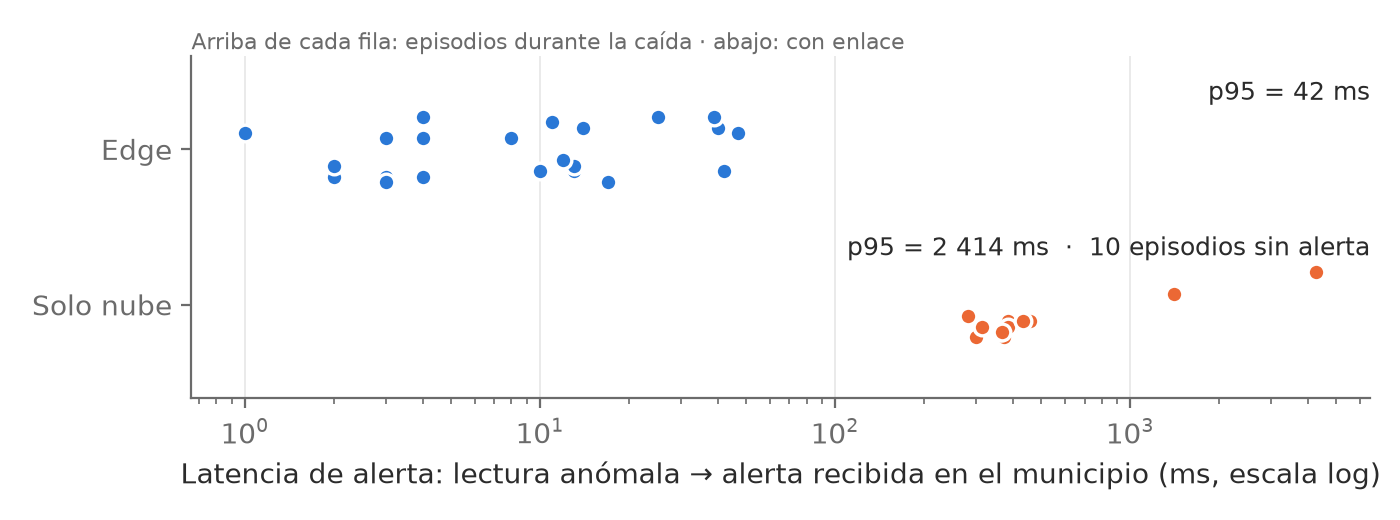
\includegraphics[width=\textwidth]{figuras/fig_latencia_alertas.png}
  \caption{Latencia de alerta por episodio detectado (escala logarítmica). Los
  diez episodios que la línea base no detecta ocurrieron durante la caída.}
  \label{fig:latencia}
\end{figure}

\begin{figure}[htbp]
  \centering
  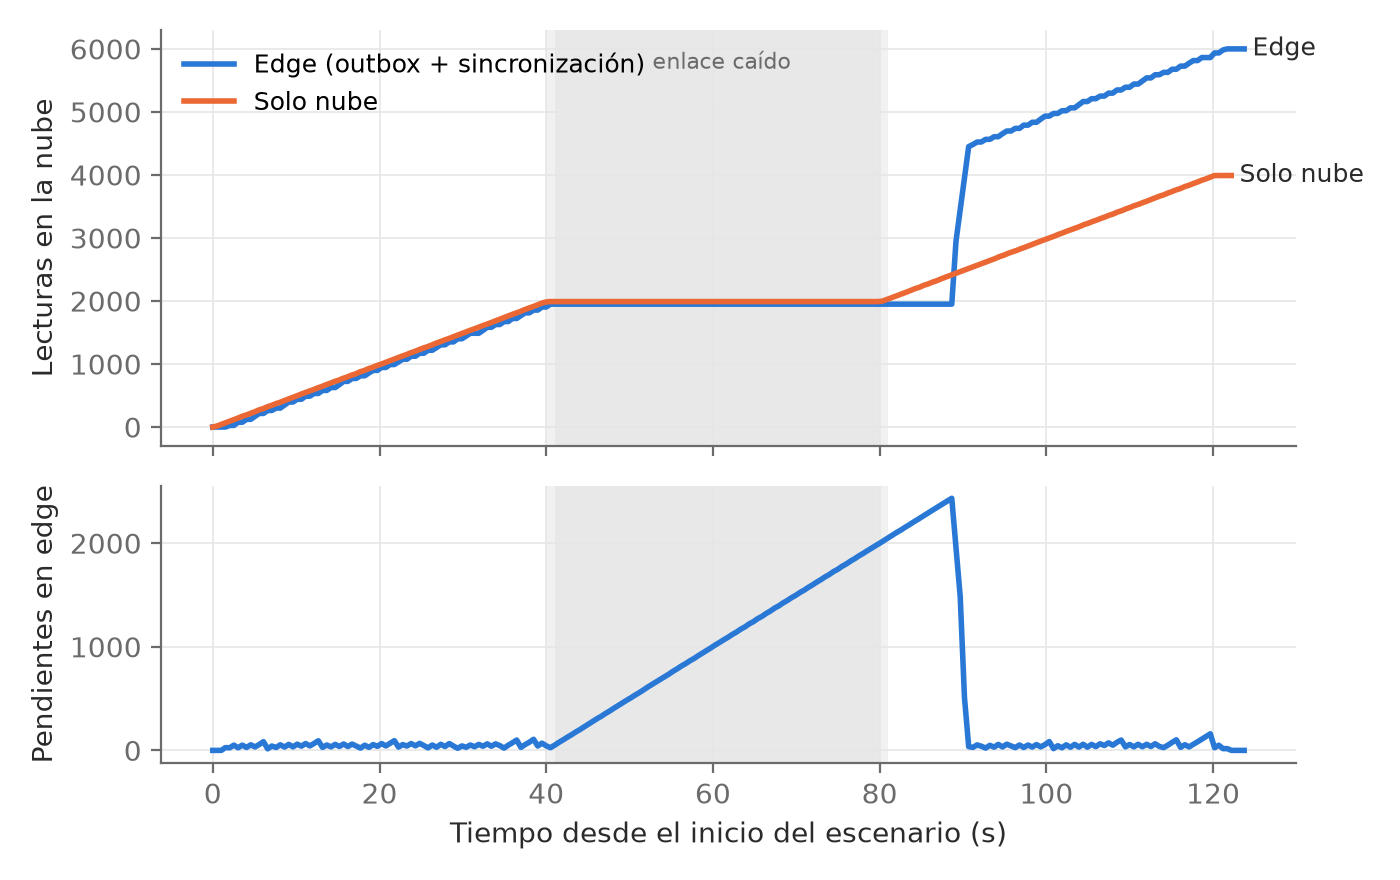
\includegraphics[width=\textwidth]{figuras/fig_linea_tiempo.png}
  \caption{Arriba: lecturas almacenadas en la nube en cada ejecución. Abajo:
  lecturas pendientes de sincronizar en el nodo \emph{edge}. La franja gris es
  la caída del enlace.}
  \label{fig:timeline}
\end{figure}

\textbf{H1 (latencia y continuidad).} Se cumple. El \emph{edge} entregó las
alertas con una mediana de 10,5\,ms y un p95 de 42\,ms (máximo 47\,ms), sin
diferencia apreciable durante la caída. La línea base tuvo una mediana de
380\,ms y un p95 de 2\,414\,ms. Con el enlace disponible su p95 fue 445\,ms,
casi todo el viaje de ida y vuelta por la WAN. Durante la caída solo generó
alerta para 2 de 12 episodios, y únicamente porque esos episodios seguían
activos cuando volvió el enlace, con 1,4 y 4,3\,s de retraso. El \emph{edge}
detectó los 24 episodios (19 por umbral y 5 crecidas súbitas por z-score), sin
falsas alarmas en ninguna de las dos ejecuciones.

\textbf{H2 (sin pérdida).} Se cumple. La nube terminó con las 6\,000 lecturas
producidas en la ejecución \emph{edge}. La línea base perdió 2\,009 (33,5\,\%):
todo lo producido durante los 40\,s de caída.

\textbf{H3 (sin duplicados).} Se cumple. Las diez pérdidas de ACK inyectadas
provocaron el reenvío de 502 lecturas que la nube ya tenía; todas fueron
reconocidas como duplicadas y no se almacenó ninguna dos veces.

\textbf{H4 (convergencia).} Se cumple, con un hallazgo de diseño. El
\emph{backlog} llegó a 2\,433 lecturas y volvió a su nivel normal (p95 de 88
pendientes con enlace) 9,7\,s después de la reconexión. De ese tiempo, 8,1\,s
transcurrieron antes del primer reintento exitoso, porque el agente estaba en
la espera máxima del \emph{backoff}; el vaciado como tal tomó cerca de 1,6\,s.
El tope del \emph{backoff} es, por tanto, el parámetro que domina la
convergencia. Un sondeo liviano del enlace mientras se espera reduciría ese
tiempo sin volver a saturar la red.

\textbf{H5 (auditoría).} Se cumple. La cadena de 116 entradas se verificó
íntegra. Al alterar la entrada 58 en una copia de la base, la verificación la
señaló como la primera entrada inválida. La cadena la escribe el nodo
\emph{edge} en Java y la verifica un programa independiente en Python, lo que
confirma además que el formato es reproducible fuera del sistema que lo genera.

\textbf{Capacidad.} Con 500 mensajes por segundo el \emph{edge} procesó las
20\,000 lecturas sin acumular cola, con un tiempo de procesamiento por mensaje
de 0,26\,ms (p95) y 0,52\,ms (p99), una latencia de alerta p95 de 6,4\,ms y
todos los episodios detectados.

\subsection{Validación con la nube desplegada en AWS}
\label{sec:prototipo-aws}

Para comprobar que los resultados no dependen de la WAN emulada, la API de la
nube se desplegó en una instancia EC2 de AWS (Amazon Linux 2023, t3.medium,
región us-east-1, en el AWS Academy Learner Lab). El nodo \emph{edge}, el
broker, el emulador del enlace y el simulador siguieron en el portátil, que
hace las veces de puesto de mando municipal. Así, el enlace \emph{edge}--nube
atraviesa internet de verdad: el emulador queda con latencia y jitter en cero y
solo se usa para cortar el enlace de forma controlada. El \emph{security group}
de la instancia admite conexiones únicamente desde la IP pública del puesto de
mando, y un script de PowerShell enciende la instancia, actualiza esa regla y
levanta el entorno local en cada sesión, porque el laboratorio apaga la
instancia y cambia su IP al terminar.

La tabla~\ref{tab:resultados-aws} compara el mismo experimento con la WAN
emulada y con la nube en AWS.

\begin{table}[htbp]
\centering
\caption{Mismo experimento con WAN emulada (200\,$\pm$\,80\,ms por sentido) y con
la nube desplegada en AWS (internet real hasta us-east-1).}
\label{tab:resultados-aws}
\small
\begin{tabular}{@{}lrrrr@{}}
\toprule
& \multicolumn{2}{c}{\textbf{Solo nube}} & \multicolumn{2}{c}{\textbf{Edge}} \\
\cmidrule(lr){2-3}\cmidrule(l){4-5}
\textbf{Métrica} & \textbf{Emulada} & \textbf{AWS} & \textbf{Emulada} & \textbf{AWS} \\
\midrule
Lecturas perdidas (de 6\,000) & 2\,009 & 1\,999 & 0 & 0 \\
Episodios detectados & 14/24 & 14/24 & 24/24 & 24/24 \\
Detectados durante la caída & 2/12 & 2/12 & 12/12 & 12/12 \\
Latencia de alerta p50 (ms) & 380 & 129 & 10,5 & 8 \\
Latencia de alerta p95 (ms) & 2\,414 & 2\,615 & 42 & 36 \\
Duplicados almacenados en la nube & 0 & 0 & 0 & 0 \\
Vaciado del \emph{backlog} (s) & -- & -- & 9,7 & 2,4 \\
\bottomrule
\end{tabular}
\end{table}

Las cinco hipótesis se mantienen con la nube real. La latencia de la línea base
es menor que con la WAN emulada (mediana de 129\,ms frente a 380\,ms), porque el
viaje de ida y vuelta real hasta us-east-1 resultó más corto que los 400\,ms
emulados; aun así es más de un orden de magnitud mayor que la del \emph{edge},
y la caída le sigue costando un tercio de las lecturas y 10 de los 12
episodios. El vaciado más rápido del \emph{backlog} no es una mejora del
sistema: en esa ejecución el primer reintento exitoso llegó 1,7\,s después de
la reconexión, frente a 8,1\,s, según en qué punto de la espera del
\emph{backoff} estaba el agente. El hallazgo de H4 sigue vigente.

\subsection{Limitaciones y amenazas a la validez}

\begin{itemize}[leftmargin=*]
  \item Las mediciones principales corrieron en un solo equipo; la
        validación de la sección~\ref{sec:prototipo-aws} llevó la nube a AWS,
        pero el nodo \emph{edge}, el broker y los dispositivos simulados
        siguieron en el mismo equipo. La red local entre campo y \emph{edge}
        no tiene latencia; en una red de radio real se sumarían decenas a
        cientos de milisegundos a la latencia del \emph{edge}, que seguiría
        lejos de la línea base y, sobre todo, no dependería de la WAN.
  \item Los datos son sintéticos y los episodios son claros. Las cifras de
        precisión y \emph{recall} prueban que el flujo funciona, no la calidad
        del detector frente a señales reales; para eso hacen falta series
        históricas de estaciones del IDEAM o de redes de monitoreo locales.
  \item La línea base no almacena lecturas en el dispositivo durante la caída.
        Si lo hiciera, evitaría la pérdida de datos pero sus alertas
        llegarían, como mínimo, con el retraso de la caída completa.
  \item SQLite en modo WAL con \texttt{synchronous=NORMAL} resiste la caída del
        proceso pero no un corte de energía del equipo; en producción el nodo
        usaría PostgreSQL con escritura sincrónica.
  \item Solo se modeló un nodo \emph{edge}. Varios municipios sincronizando a
        la vez y la resolución de conflictos sobre datos editados en ambos
        lados quedan como trabajo siguiente.
\end{itemize}

\subsection{Reproducibilidad}

El código fuente acompaña este documento: es un proyecto Maven multimódulo
cuya raíz contiene el \texttt{pom.xml}, el \emph{wrapper} \texttt{mvnw}, los
módulos \texttt{shared/}, \texttt{edge-node/} y \texttt{cloud-api/}, y las
herramientas de prueba en Python. \texttt{mvnw verify} ejecuta las pruebas
unitarias (JUnit). \texttt{docker compose up -{}-build} levanta el broker, el
nodo \emph{edge}, el enlace emulado y la nube. \texttt{docker compose -{}-profile
experiment run -{}-rm experiment} repite el experimento completo y regenera la
tabla~\ref{tab:resultados} y las figuras~\ref{fig:latencia}
y~\ref{fig:timeline}. Sin Docker, \texttt{mvnw package} seguido de
\texttt{python scripts/run\_local\_stack.py} levanta los mismos servicios como
procesos locales. Con la nube en AWS, \texttt{scripts/aws-up.ps1} enciende la
instancia y levanta el resto con \texttt{docker-compose.aws.yml}; el
procedimiento está en \texttt{docs/aws/despliegue-aws.md}. El tablero del COP
local queda en \texttt{http://localhost:8080}.


% =====================================================================
\section{Contribución, métricas y trabajos futuros}
% =====================================================================

\subsection{Contribución}

\begin{table}[htbp]
\centering
\caption{Situación actual, propuesta arquitectónica y resultado esperado.}
\label{tab:contribucion}
\begin{tabularx}{\textwidth}{@{}LLL@{}}
\toprule
\textbf{Situación} & \textbf{Propuesta} & \textbf{Resultado} \\
\midrule
Información distribuida     & Interoperabilidad        & Visión común \\
Evaluación manual           & IA + imágenes            & Evaluación preliminar rápida \\
Asignación subjetiva        & Optimización + experto   & Decisiones cuantificables \\
Rutas estáticas             & Optimización dinámica    & Mejor logística \\
Dependencia de conectividad & Edge/\emph{offline-first} & Resiliencia \\
Sistemas aislados           & \emph{System of Systems} & Coordinación \\
Decisiones no trazables     & Auditoría                & Transparencia \\
Recursos limitados          & Priorización por impacto & Mejor asignación \\
\bottomrule
\end{tabularx}
\end{table}

\subsection{Métricas}
\label{sec:metricas}

\begin{itemize}[leftmargin=*]
  \item \textbf{Eficiencia:} reducción del tiempo de asignación, llegada,
        kilómetros y costos.
  \item \textbf{Cobertura:} población prioritaria atendida, necesidades
        satisfechas e infraestructura crítica cubierta.
  \item \textbf{Resiliencia:} disponibilidad, latencia y porcentaje de
        operaciones \emph{offline}. El prototipo de la
        sección~\ref{sec:prototipo} ya mide latencia de alerta, pérdida de
        datos, duplicados y tiempo de convergencia bajo una caída del enlace.
  \item \textbf{IA:} precisión, \emph{recall}, F1-score, falsos positivos y
        tiempo de procesamiento.
  \item \textbf{Gobernanza:} decisiones auditables, recursos trazables y
        tiempo para reconstruir decisiones.
\end{itemize}

\subsection{Trabajos futuros}

\begin{enumerate}[leftmargin=*]
  \item Llevar el prototipo a varios nodos \emph{edge} sincronizando a la vez,
        con resolución de conflictos. La nube ya se desplegó en una instancia
        EC2 de AWS (sección~\ref{sec:prototipo-aws}); el siguiente paso es
        reemplazar SQLite por una base gestionada y exponer la API detrás de
        un balanceador con TLS y autenticación.
  \item Validar el detector con series reales de estaciones hidrometeorológicas
        y sísmicas, e integrar un modelo entrenado en el mismo punto del flujo.
  \item Integrar sistemas nacionales y regionales existentes.
  \item Desarrollar modelos especializados por tipo de desastre.
  \item Usar imágenes SAR para escenarios con nubosidad.
  \item Incorporar drones y nuevas fuentes de observación.
  \item Desarrollar modelos predictivos de necesidades.
  \item Construir gemelos digitales de territorios críticos.
  \item Simular escenarios y comparar estrategias.
  \item Fortalecer gobernanza e intercambio de datos.
  \item Evaluar económicamente estrategias preventivas frente a reactivas.
  \item Aprender de emergencias anteriores.
\end{enumerate}

Una línea especialmente relevante sería desarrollar un gemelo digital regional
que permita simular escenarios y estimar cómo cambian los resultados según la
ubicación de recursos, disponibilidad de vías, condiciones meteorológicas y
distribución de la población.

% =====================================================================
\section{Conclusiones}
% =====================================================================

La respuesta efectiva ante desastres no depende únicamente de disponer de más
datos ni de incorporar inteligencia artificial. El reto consiste en integrar
organizaciones, procesos, información y tecnología para convertir datos
heterogéneos en decisiones oportunas, coordinadas y trazables.

La arquitectura propuesta aborda este reto mediante interoperabilidad,
capacidades geoespaciales, IA para evaluación preliminar, optimización
logística, operación resiliente y gobernanza. No busca reemplazar todos los
sistemas existentes, sino conectarlos dentro de una arquitectura común.

La documentación en notación C4 complementa la propuesta: traduce las capas de
negocio, información, aplicaciones y tecnología en contenedores y componentes
concretos, deja explícito dónde interviene la persona que decide y muestra, en
el diagrama de despliegue, cómo se sostiene la operación cuando falla la
conectividad.

El prototipo convierte esa promesa en evidencia medible. Con el enlace caído,
el nodo \emph{edge} siguió detectando y alertando en milisegundos, conservó
todas las lecturas y las entregó a la nube sin duplicados al reconectarse. La
alternativa centralizada perdió un tercio de los datos y casi todas las
alertas de la caída. El experimento también mostró que el tope del
\emph{backoff} domina el tiempo de convergencia, un parámetro que la
arquitectura debe ajustar de forma explícita. Con la nube desplegada en AWS y
el enlace sobre internet real, las conclusiones se mantuvieron.

La tesis central es que una respuesta moderna a desastres debe entenderse como
un sistema de sistemas. La combinación de Arquitectura Empresarial,
interoperabilidad, GIS, IA, optimización matemática, resiliencia tecnológica y
gobernanza puede mejorar la coordinación y proporcionar una base medible para
implementaciones regionales o nacionales.

% =====================================================================
\section*{Referencias iniciales}
\addcontentsline{toc}{section}{Referencias iniciales}
% =====================================================================

\begin{itemize}[leftmargin=*]
  \item Mani, Z. A., Sultan, M. A. S., Plummer, V., \& Goniewicz, K. (2023).
        \emph{Navigating Interoperability in Disaster Management}.
        International Journal of Disaster Risk Science, 14, 873--885.
  \item Kaur, N., Lee, C.-C., Mostafavi, A., \& Mahdavi-Amiri, A. (2022).
        \emph{Large-scale Building Damage Assessment using a Novel
        Hierarchical Transformer Architecture on Satellite Images}.
  \item Alisjahbana, I., Li, J., Strong, B., \& Zhang, Y. (2024).
        \emph{DeepDamageNet: A two-step deep-learning model for
        multi-disaster building damage segmentation and classification using
        satellite imagery}.
  \item Shehadeh, K. S., \& Tucker, E. L. (2020). \emph{Stochastic
        Optimization Models for Location and Inventory Prepositioning of
        Disaster Relief Supplies}.
  \item Maroof, A., et al. (2023). \emph{Vehicle Routing Optimization for
        Humanitarian Supply Chain: A Systematic Review}. IEEE Access, 11,
        127157--127175.
  \item Bonfanti, R. C., et al. (2024). \emph{The Role of Trust in Disaster
        Risk Reduction: A Critical Review}.
  \item Copernicus Emergency Management Service (CEMS). Documentación sobre
        información geoespacial para gestión de emergencias.
  \item Unidad Nacional para la Gestión del Riesgo de Desastres (UNGRD).
        \emph{Sistema Nacional de Información para la Gestión del Riesgo de
        Desastres}.
  \item United Nations Office for Disaster Risk Reduction (UNDRR).
        \emph{Sendai Framework for Disaster Risk Reduction 2015--2030}.
\end{itemize}

\end{document}
